\chapter[Xây dựng ứng dụng\\tìm kiếm đối tượng trên ảnh]{Xây dựng ứng dụng\\tìm kiếm đối tượng trên ảnh}
\label{chapter:application}
\ifpdf
    \graphicspath{{Chapter5/Chapter5Figs/PNG/}{Chapter5/Chapter5Figs/PDF/}{Chapter5/Chapter5Figs/}}
\else
    \graphicspath{{Chapter5/Chapter5Figs/EPS/}{Chapter5/Chapter5Figs/}}
\fi
\markboth{\MakeUppercase{\thechapter. Xây dựng ứng dụng tìm kiếm đối tượng trên ảnh}}{\thechapter. Xây dựng ứng dụng tìm kiếm đối tượng trên ảnh}

Trên cơ sở các phương pháp đã nghiên cứu và những kết quả thực nghiệm của phương pháp đề xuất, chúng tôi tiến hành xây dựng ứng dụng tìm kiếm đối tượng trên ảnh nhằm thực nghiệm phương pháp đề xuất trên môi trường thực tế chứng minh tính thực tiễn của đề tài.

Trong chương này, trước tiên chúng tôi sẽ giới thiệu tổng quan về mục đích và các chức năng chính của ứng dụng (mục \ref{c5-tongquan}). Sau đó là bước thiết kế kiến trúc, tổ chức các thành phần và giao diện của ứng dụng (mục \ref{c5-thietke}). Cuối cùng là bước cài đặt, thử nghiệm và đánh giá kết quả của hệ thống đã cài đặt (mục \ref{c5-caidat}).

\section{Tổng quan ứng dụng}
\label{c5-tongquan}

	\subsection{Mục đích và phạm vi của ứng dụng}
Như đã giới thiệu trong mục \ref{section:intro-problem}, các hệ thống truy vấn ảnh có vô vàn ứng dụng khác nhau trong thực tế. Trong đề tài này, chúng tôi xây dựng ứng dụng nhằm phục vụ mục đích cơ bản là tìm kiếm đối tượng trên những kho dữ liệu ảnh với kích thước có thể lên tới hàng trăm ngàn ảnh. Đó có thể là kho dữ liệu ảnh của một tổ chức, công ty về một lĩnh vực nào đó. Hay xa hơn, ứng dụng này có thể phát triển cho việc tìm kiếm đối tượng trên kho dữ liệu video vì ta hoàn toàn có thể rút trích được hình ảnh từ các frame của video.

Hơn nữa, ngày nay điện thoại thông minh đang dần trở lên rất phổ biến và dần trở thành vật bất ly thân của con người. Các ứng dụng trên điện thoại thông minh cũng phát triển ồ ạt, cung cấp cho người dùng rất nhiều tiện ích. Vì vậy chúng tôi hướng tới một ứng dụng giao tiếp với người dùng trên nền tảng điện thoại thông minh sử dụng hệ điều hành Android. Và để gần hơn với các yêu cầu thực tế khi số lượng người dùng ngày càng tăng, chúng tôi đề xuất xây dựng một hệ thống xử lý đám mây với nhiều server xử lý, kết nối với nhau thông qua dịch vụ web (web service).
	
	\subsection{Các chức năng chính}
Ứng dụng được xây dựng với mục tiêu cung cấp một hệ thống tìm kiếm đối tượng trên ảnh, nhận đầu vào là hình ảnh chứa đối tượng truy vấn và trả về danh sách xếp hạng các hình ảnh theo mức độ tương đồng với hình truy vấn. Chi tiết các chức năng chính của ứng dụng như sau:

\begin{itemize}

\item Chụp hình đối tượng: người dùng có thể sử dụng camera của điện thoại để chụp hình đối tượng và tìm kiếm.

\item Chọn ảnh được lưu trữ trước trong máy: người dùng có thể chọn một ảnh có chứa đối tượng được lưu trữ trong điện thoại, thẻ nhớ để tìm kiếm.

\item Chọn vùng đối tượng: để nâng cao độ chính xác của việc tìm kiếm, người dùng có thể khoanh vùng đối tượng cần tìm trên ảnh.

\item Xem và tương tác với kết quả truy vấn: hiển thị kết quả truy vấn là danh sách các hình ảnh và cho phép người dùng xem và tải xuống các hình ảnh này.

\end{itemize}

\section{Xây dựng ứng dụng}
\label{c5-thietke}

	\subsection{Kiến trúc tổng quan}
Kiến trúc của hệ thống gồm làm 3 thành phần chính:

\begin{itemize}

\item \textbf{Client side:} là một ứng dụng trên điện thoại di động sử dụng hệ điều hành Android, cung cấp giao diện để người dùng tương tác trực tiếp với hệ thống tìm kiếm đối tượng trên ảnh.

\item \textbf{Web service:} là thành phần trung gian, nhận các yều cầu từ phía client. Thực hiện điều phối và cân bằng tải, chuyển tiếp các yêu cầu từ người dùng tới các server xử lý, đồng thời tiếp nhận kết quả xử lý và trả về cho từng client tương ứng.

\item \textbf{Server side:} là thành phần xử lý chính của hệ thống, nhận yêu cầu từ web service chuyển tiếp tới, xử lý và trả về kết quả cho web service. Chi phí xử lý truy vấn hình ảnh tại server rất lớn, do đó để đảm bảo yêu cầu thực tế, hệ thống có thể sử dụng nhiều server để xử lý đồng thời các yêu cầu.

\end{itemize}

Hình \ref{FigArchitecture} minh họa cho mô hình hoạt động tổng quan của hệ thống.

Chi tiết các thành phần được trình bày trong các phần tiếp theo (\ref{subsection:server_side}, \ref{subsection:web_service} \ref{subsection:client_side}).

\begin{figure}[!htbp]
  \begin{center}
    \leavevmode
    \ifpdf
      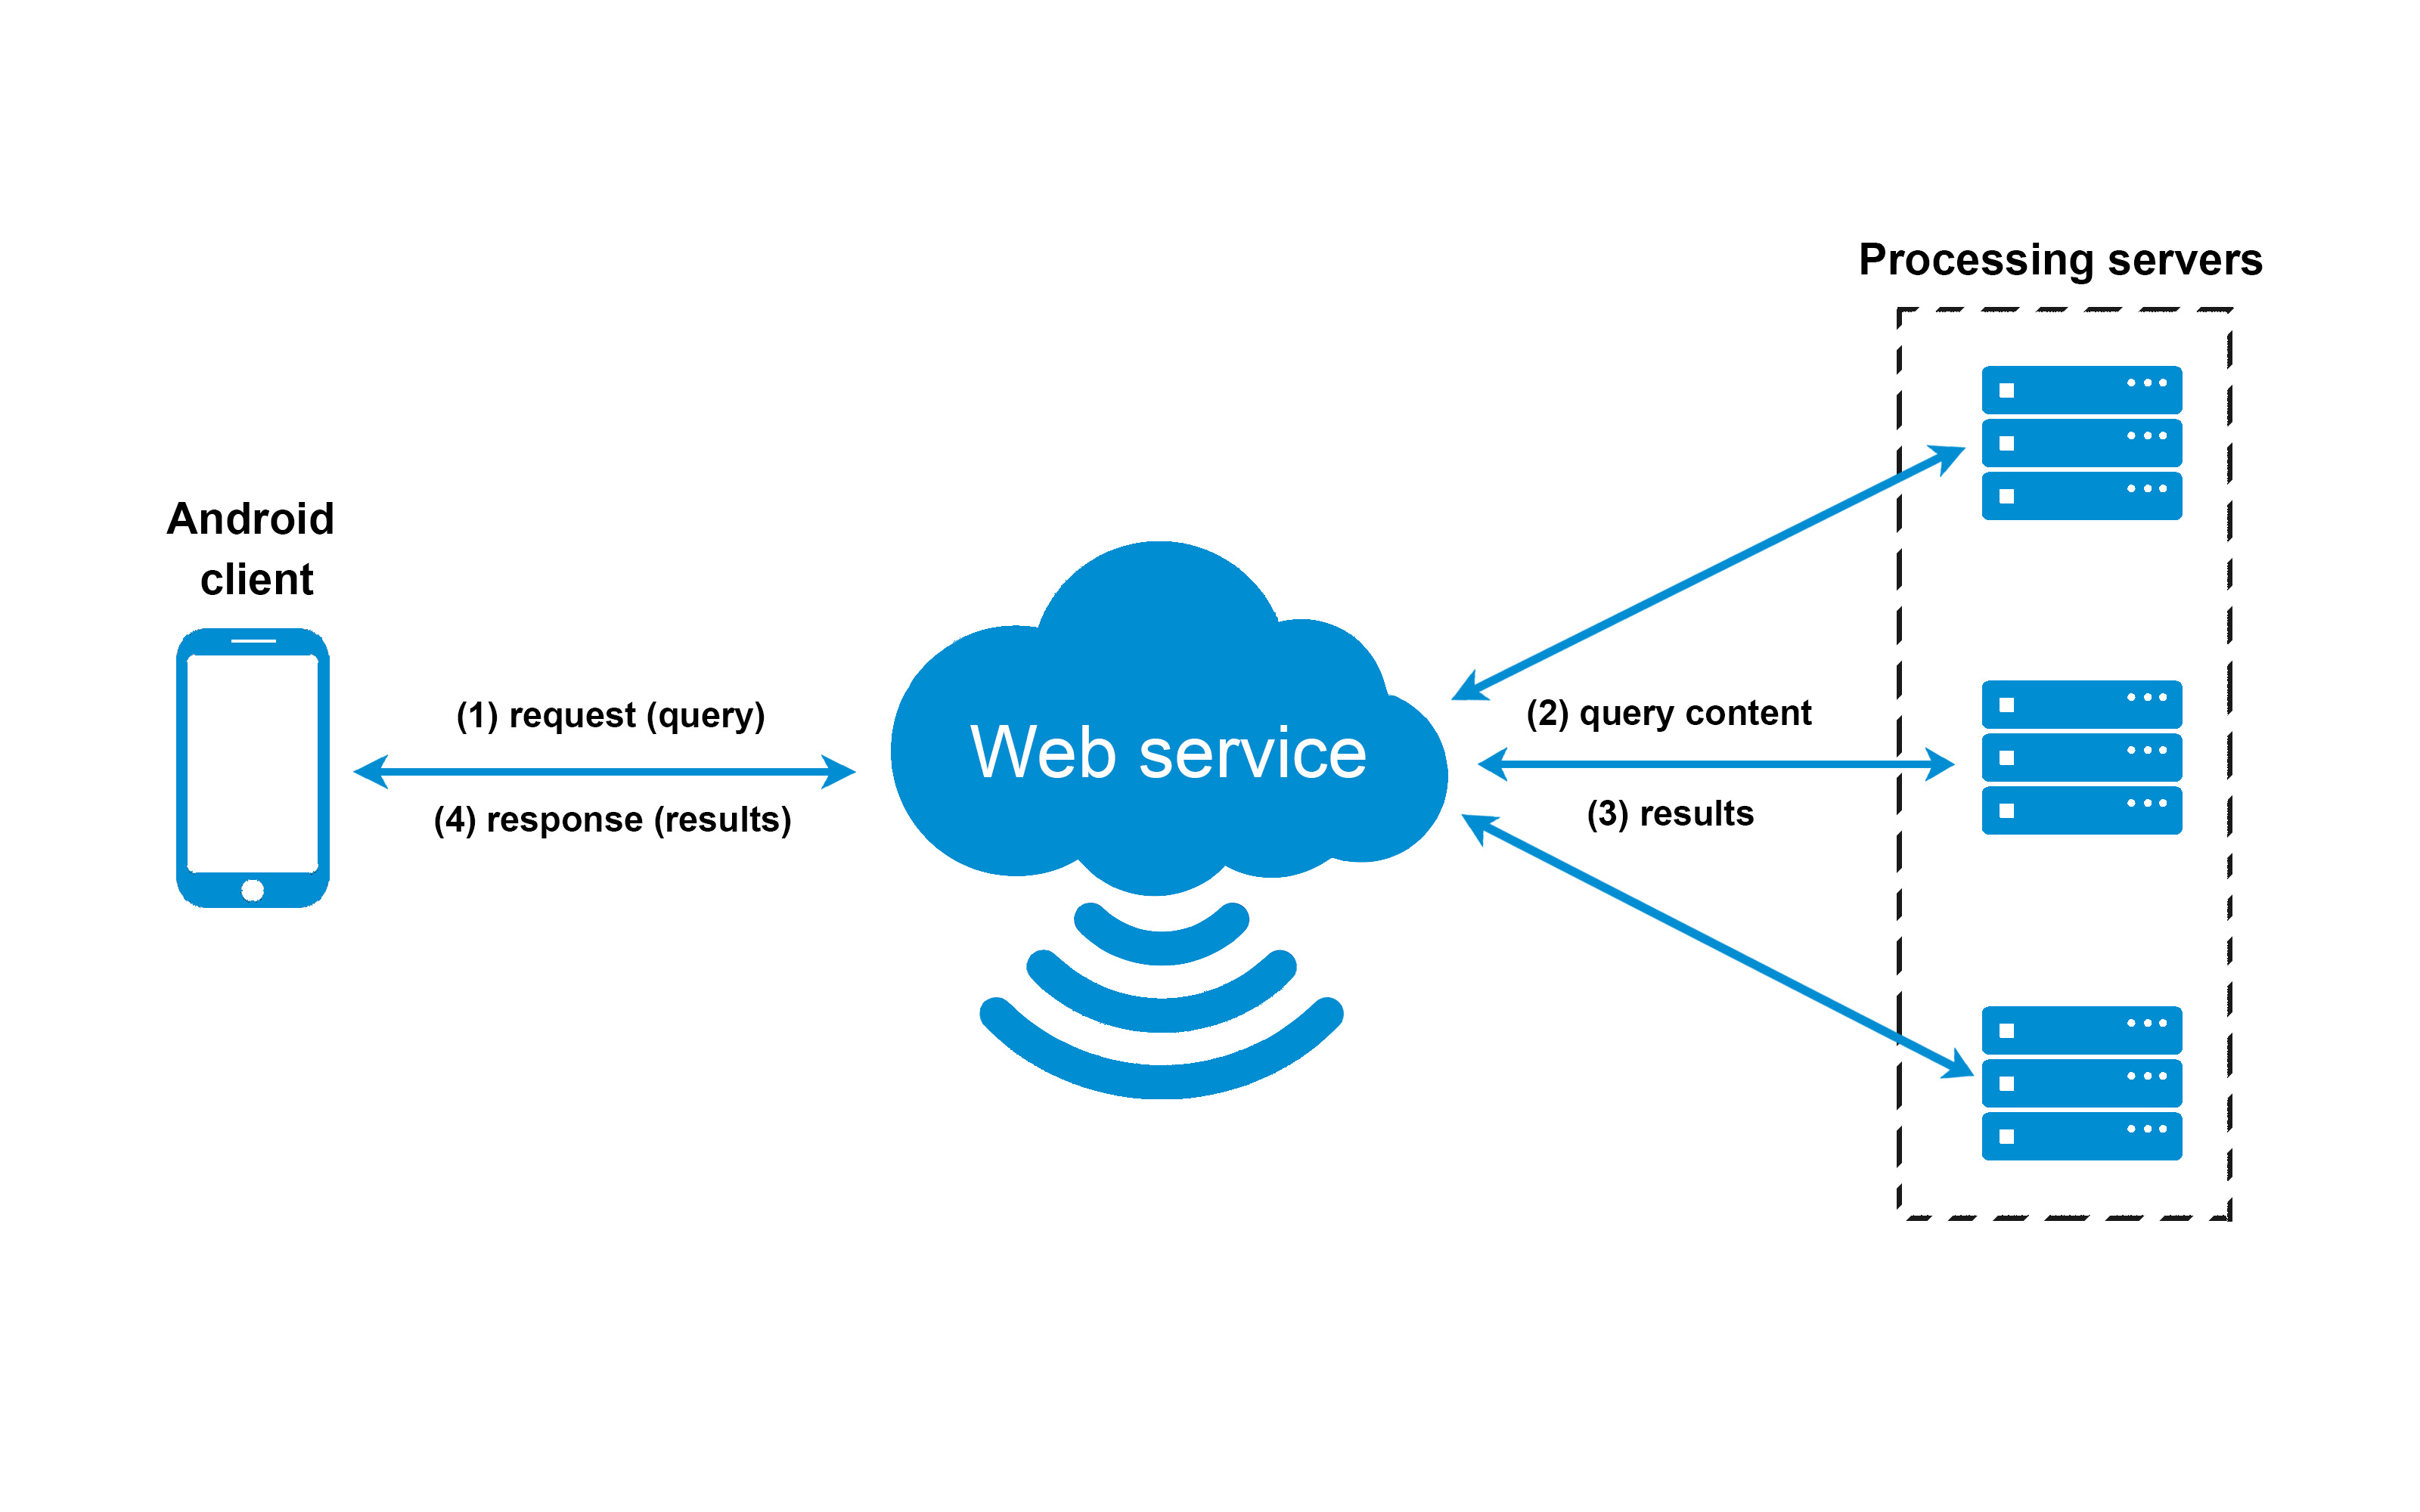
\includegraphics[scale=0.12]{architecture}
    \else
      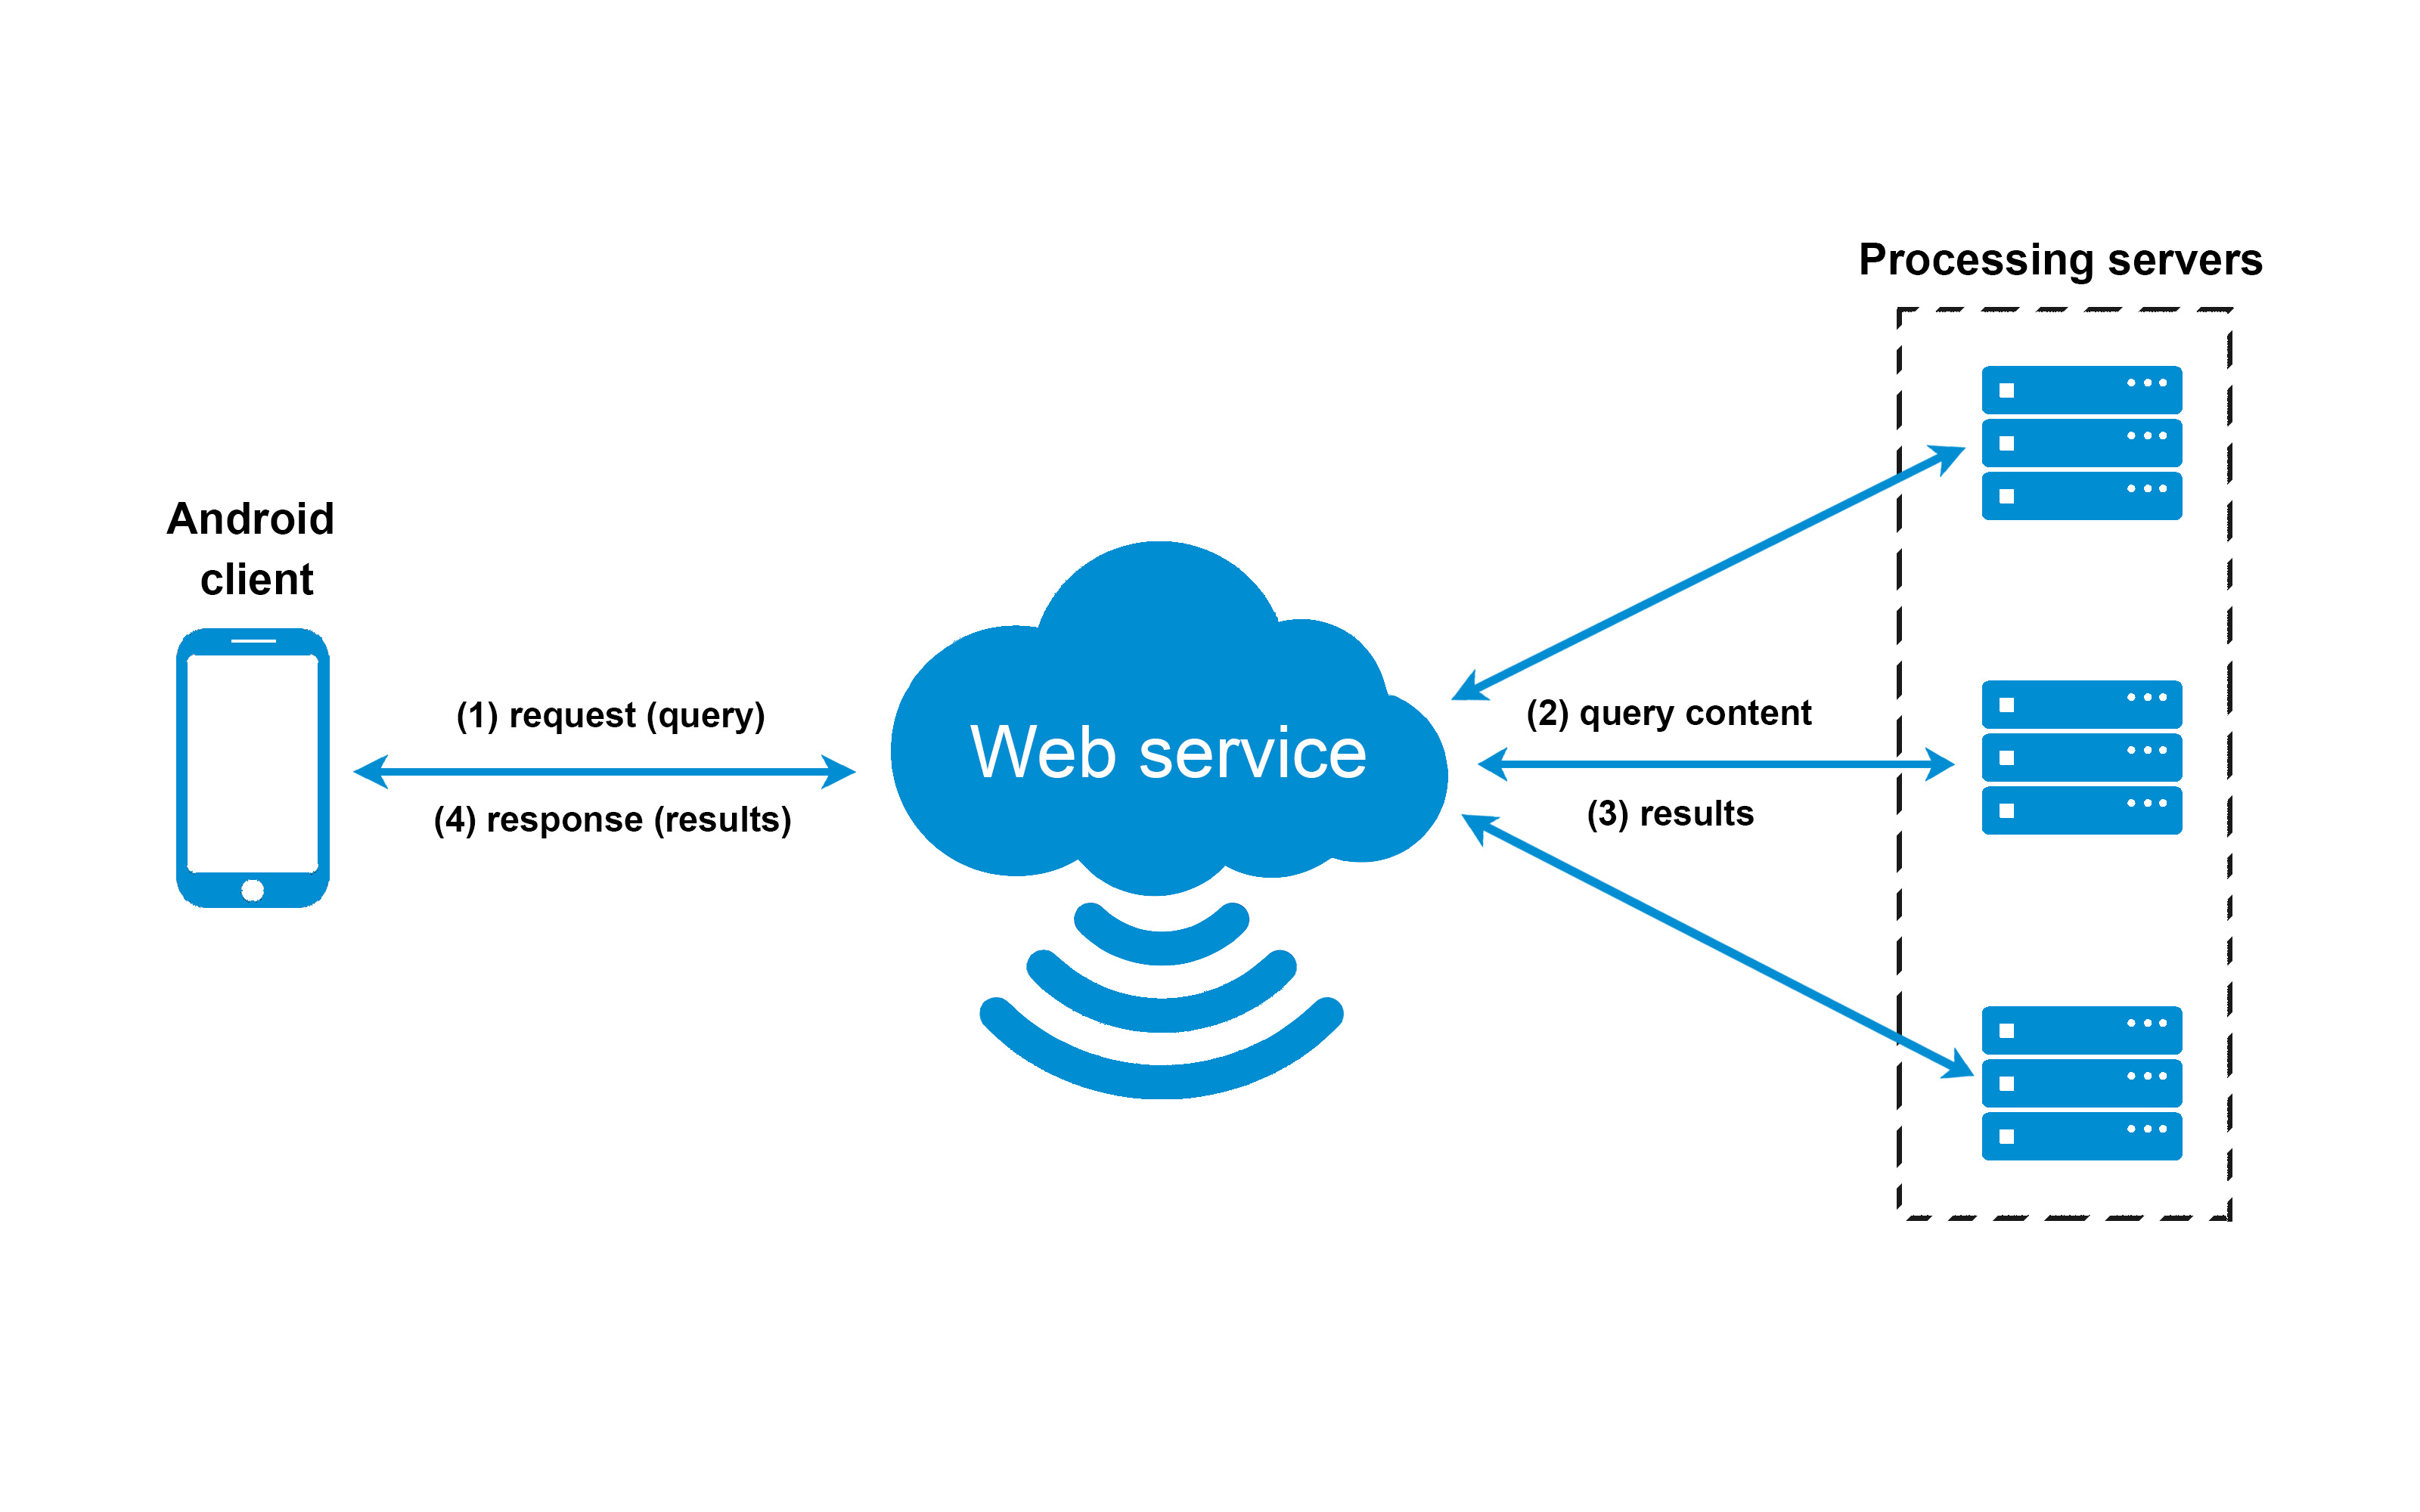
\includegraphics[scale=0.12]{architecture}
    \fi
    \caption[Kiến trúc tổng quan của hệ thống]{Kiến trúc tổng quan của hệ thống.}
    \label{FigArchitecture}
  \end{center}
\end{figure}

\subsection{Server side}
\label{subsection:server_side}
Server side chính là thành phần quan trọng nhất của hệ thống, thực hiện các tác vụ xử lý truy vấn. Cấu trúc của server side gồm hai thành phần chính tương ứng với hai quá trình xử lý là quá trình training và quá trình truy vấn.

\begin{itemize}
\item \textbf{Quá trình training:} là quá trình biểu diễn lại tập dữ liệu hình ảnh, sử dụng các mô hình biểu diễn hình ảnh kết hợp với các phương pháp, kỹ thuật khác với mục đích tạo ra các dữ liệu cần thiết phục vụ quá trình truy vấn.

\item \textbf{Quá trình truy vấn:} là quá trình tương tác trực tiếp với hệ thống tìm kiếm đối tượng trên ảnh, nhận đầu vào là một hình ảnh, thực hiện các bước xử lý truy vấn ảnh và trả về kết quả là một tập các hình ảnh được sắp xếp theo thứ tự có độ tương đồng với hình ảnh truy vấn giảm dần.
\end{itemize}

\subsubsection{Quá trình training}
Như đã trình bày sơ lược trong mục trong mục \ref{sec:inverted-index} và \ref{experimental-setting}, quá trình training bao gồm các bước sau:

\textbf{Dò tìm, phát hiện và rút trích đặc trưng.} Từ kho dữ liệu hình ảnh được lưu sẵn trên server, bước đầu tiên của quá trình xử lý là sử dụng phương pháp phát hiện keypoint Hessian-Affine để xác định được vị trí các điểm keypoint trên hình ảnh. Từ thông tin đó, bộ SIFT descriptor mô tả và rút trích được 1 vector 128 chiều tương ứng với mỗi điểm keypoint. Những vector này sẽ được tính toán lại bằng phương pháp RootSIFT\cite{philbin2007object}. Các vector thu được chính là các tập đặc trưng của hình ảnh. 

\textbf{Gom cụm đặc trưng và xây dựng từ điển.} Các vector đặc trưng sẽ được gom cụm bằng thuật toán Approximate K-Means\cite{philbin2007object} để thu được các visual word với số lượng cụm là k = 1 triệu. Kết quả ta sẽ thu được các visual word để mô tả hình ảnh. Từ những visual word này, ta sẽ xây dựng thành một từ điển để phục vụ cho việc biểu diễn hình ảnh khi truy vấn.

\textbf{Xây dựng chỉ mục ngược.} Theo như phương pháp đề xuất đã được đề cập chi tiết trong Chương \ref{chapter:proposed}, chúng tôi sẽ xây dựng chỉ mục ngược từ từ điển nhằm đạt được hiệu suất cao trong quá trình truy vấn. Cụ thể hơn, từ bộ từ điển và thông tin không gian của tất cả các visual word của mỗi hình ảnh trong bộ dữ liệu, với cấp độ phân cấp là 2, có 21 chỉ mục ngược sẽ được tạo ra và lưu vào một file.

Sơ đồ xử lý cùng các thông số cài đặt được trình bày chi tiết trong phần cài đặt thí nghiệm (Mục \ref{experimental-setting}) và trong Hình \ref{FigInvertedFile}. Quá trình training được thực hiện độc lập trên server và là bước tiền đề, tạo dữ liệu phục vụ cho quá trình truy vấn.

\subsubsection{Quá trình truy vấn}
\label{subsubsection:truyvan_server}
Đây là quá trình tương tác trực tiếp với hệ thống tìm kiếm và chạy song song web service, nhận yêu cầu từ web service chuyển tiếp tới sau đó tiến hành truy vấn trả kết quả ngược trở lại web service.

Ngày nay, chất lượng hình ảnh ngày càng được tăng cao, kéo theo dung lượng hình ảnh cũng rất lớn. Việc trả về cho client một lượng lớn hình ảnh chất lượng cao là không thể vì lưu lượng và tốc độ băng thông còn bị giới hạn rất nhiều. Vì vậy sau khi xử lý truy vấn, server sẽ trả về cho client một danh sách hình ảnh thu nhỏ để đảm bảo tốc độ phản hồi. Chi tiết sẽ được trình bày rõ hơn trong phần tối ưu hiệu suất hệ thống (Mục \ref{subsection:optimize}).

Việc trả về cho client các hình ảnh thu nhỏ sẽ phát sinh thêm các chức năng khác như: xem hình ảnh chất lượng tốt hơn, tải hình ảnh gốc về thiết bị. Vì vậy, tại phía server cung cấp hai chức năng chính tương ứng với hai loại yêu cầu từ phía client là yêu cầu truy vấn một hình ảnh và yêu cầu tải một (hoặc một tập) các hình ảnh theo các mức chất lượng khác nhau.

Với yêu cầu như trên, các server được chia làm 2 loại chính:

\begin{itemize}
\item \textbf{Server truy vấn:} tiếp nhận yêu cầu truy vấn hình ảnh, xử lý và trả về kết quả là danh sách xếp hạng cùng một phần các hình ảnh thu nhỏ giống với hình truy vấn nhất.

\item \textbf{Server truy xuất dữ liệu:} tiếp nhận yêu cầu truy xuất hình ảnh, trả về hình ảnh được lấy từ bộ nhớ.
\end{itemize}

\begin{figure}[!htbp]
  \begin{center}
    \leavevmode
    \ifpdf
      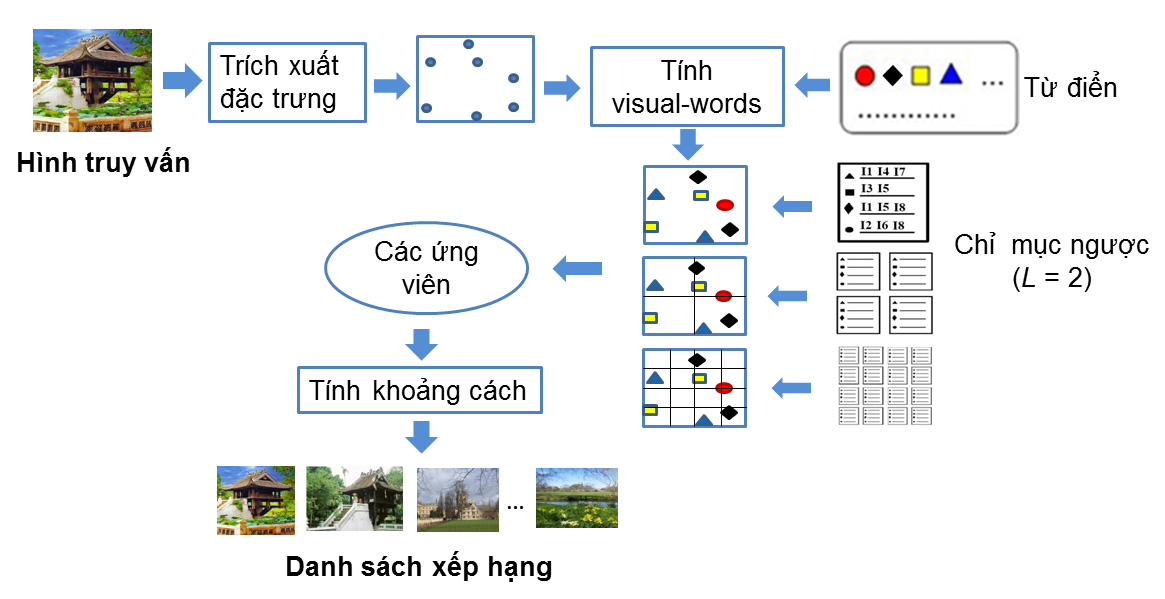
\includegraphics[scale=0.35]{query-process-server}
    \else
      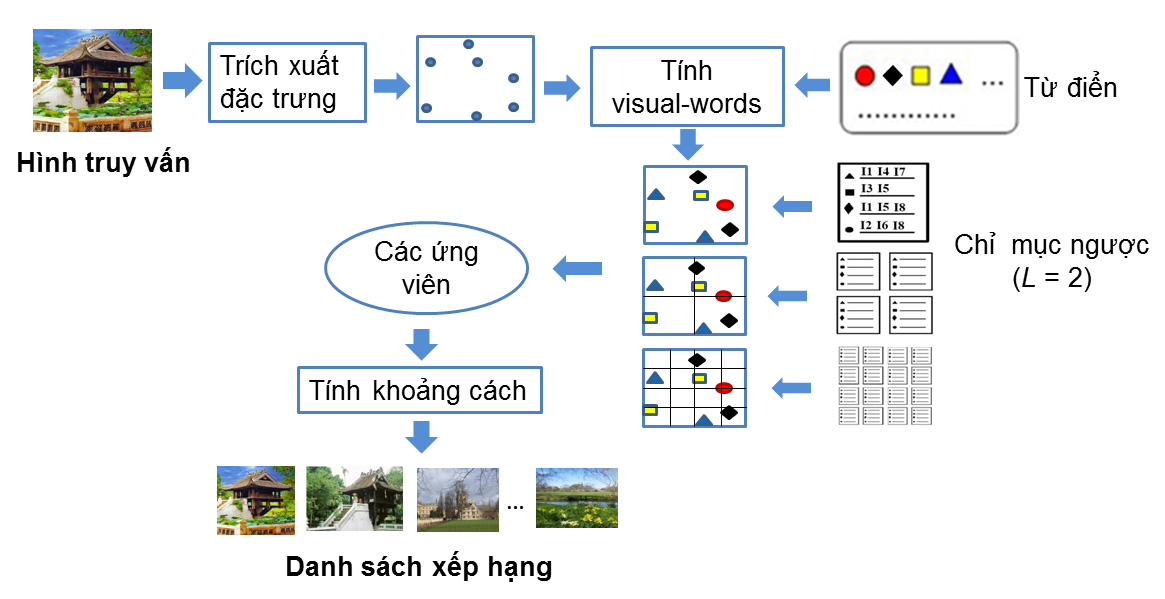
\includegraphics[scale=0.35]{query-process-server}
    \fi
    \caption[Quá trình truy vấn tại server]{Quá trình truy vấn tại server.}
    \label{query-process-server}
  \end{center}
\end{figure}

Quá trình xử lý truy vấn được đã trình bày chi tiết trong mục \ref{sec:intergrated} và được thể hiện trong Hình \ref{query-process-server}. Đầu tiên, ta sẽ rút trích đặc trưng từ hình ảnh truy vấn. Sau đó các đặc trưng này được đưa vào từ điển để lấy được các visual word tương ứng. Từ các visual word và vị trí của nó trên hình ảnh, ta sẽ dùng chỉ mục ngược đề xuất để tìm kiếm các hình ảnh ứng viên có liên quan và đồng thời tính khoảng cách từ hình truy vấn tới các hình ảnh này. Sau đó, danh sách hình ảnh ứng viên sẽ được sắp xếp theo mức độ tượng tự từ cao tới thấp. Kết quả sẽ được server gửi ngược trở về webservice và trả về cho client yêu cầu.

\subsection{Web service}
\label{subsection:web_service}
Web service là thành phần trung gian đóng vai trò phân phối các yêu cầu từ phía client tới các server xử lý. Thành phần này sử dụng dịch vụ web chạy trên các máy chủ web cung cấp các phương thức giúp client và server xử lý kết nối, truyền tải các dữ liệu cần thiết. Có nhiều cách để kết nối ba thành phần này với nhau, chi tiết sẽ được trình bày đưới đây.

Với một hệ thống tìm kiếm cơ bản sử dụng từ khóa thông thường, thành phần xử lý có thể chính là web service. Với mỗi yêu cầu tìm kiếm, nó sẽ tạo ra một tiến trình và truy xuất tới cơ sở dữ liệu để lấy thông tin một cách nhanh chóng, có thể đáp ứng nhiều yêu cầu đồng thời, phụ thuộc vào phần cứng và các thiết lập trên nó. Nhưng với một hệ thống tìm kiếm hình ảnh, chi phí tính toán và tài nguyên phục vụ quá trình tìm kiếm rất lớn, việc tạo ra nhiều tiến trình xử lý là không khả thi. Nếu giới hạn số lượng yêu cầu ở mức thấp để đảm bảo an toàn cho hệ thống thì sẽ không đáp ứng được yêu cầu thực tế, ngược lại nếu không kiểm soát các yêu cầu truy vấn thì hệ thống có thể sẽ không đáp ứng được và dễ dàng bị quá tải dẫn dến nguy hiểm cả cho phần cứng. Chính vì vậy, giải pháp tốt nhất chính là chia tải, bằng cách sử dụng nhiều server xử lý và chuyển tiếp các yêu cầu truy vấn tới các server này. Từ đó ta có hai giải pháp kết nối:

-- Giải pháp 1: Web service lưu giữ thông tin các server xử lý, khi có yêu cầu (request) từ phía client, nó sẽ gửi thông tin server để client trực tiếp kết nối và truyền tải dữ liệu tới server xử lý.

-- Giải pháp 2: Web service nhận yêu cầu từ phía client, truyền tải dữ liệu tới server xử lý, chờ kết quả xử lý từ server và gửi lại cho client. Như vậy client không được phép kết nối trực tiếp tới server xử lý.

Có thể thấy với giải pháp thứ nhất, dữ liệu qua lại trực tiếp giữa client và server nên tối ưu được quá trình truyền dẫn, không cần qua trung gian. Nhưng do client có thể nắm được thông tin của server nên nó gặp phải một vấn đề lớn là bảo mật. Vì vậy chúng tôi không sử dụng giải pháp này.

Với giải pháp thứ 2, client chỉ được phép kết nối tới web service và không hề biết thông tin của bất cứ server xử lý nào nên vấn đề bảo mật đã được giải quyết. Nhược điểm của cách này là dữ liệu phải thông qua trung gian, làm tăng thời gian truyền tải. Nhưng thường các server kết nối với nhau qua một mạng lưới internet hoặc mạng lan với tốc độ băng thông rất lớn nên thời gian truyền tải dữ liệu phần lớn phụ thuộc vào tốc độ băng thông của client. Vậy giải pháp này rõ ràng tốt hơn giải pháp đầu tiên.

Có rất nhiều cách để xây dựng một hệ thống với giải pháp trên. Một trong những cách đơn giản mà chúng tôi sử dụng là dùng web service cung cấp các phương thức để truyền tải dữ liệu giữa client và server xử lý. Cụ thể hơn, nó giống như một hệ thống chat giữa các user với nhau và web service là thành phần chuyển tiếp các thông điệp. Khi đó client và server sẽ "chat" với nhau, nhưng thông điệp ở đây phức tạp hơn. Chẳng hạn khi client truy vấn một hình ảnh, thì thông điệp ở đây là yêu cầu truy vấn kèm theo hình ảnh đã được mã hóa, và khi hoàn tất xử lý thì server sẽ gửi lại thông điệp là danh sách xếp hạng cùng cách hình ảnh.

Sơ đồ mô hình hoạt động chi tiết của web service được thể hiện trong Hình \ref{FigWS}.

\begin{figure}[!htbp]
  \begin{center}
    \leavevmode
    \ifpdf
      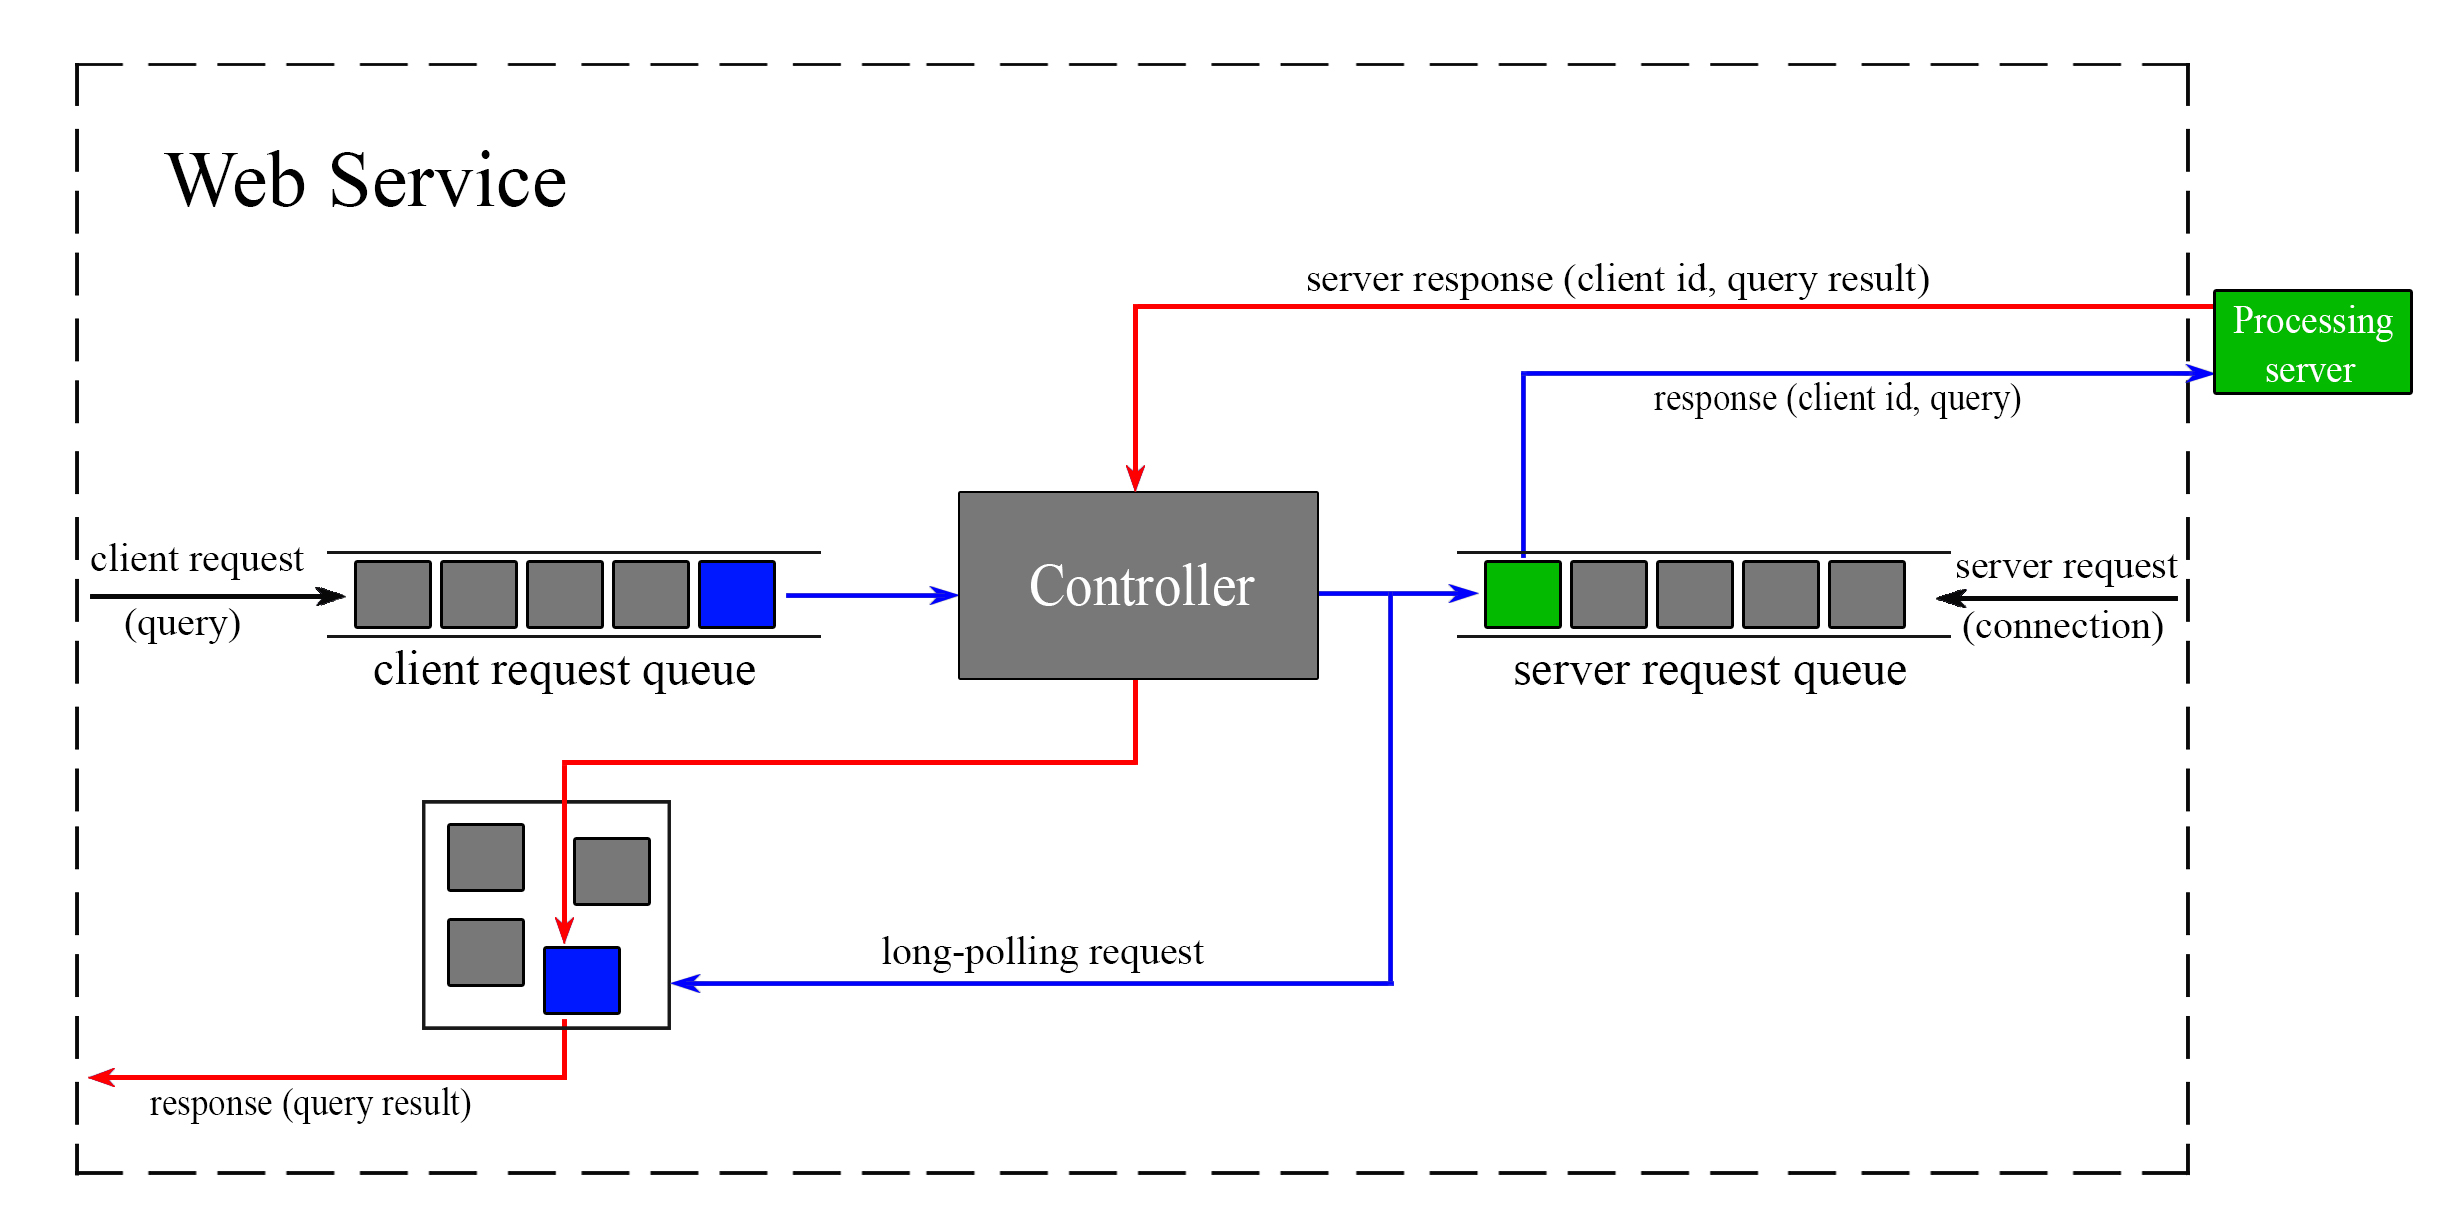
\includegraphics[scale=0.17]{ws_model}
    \else
      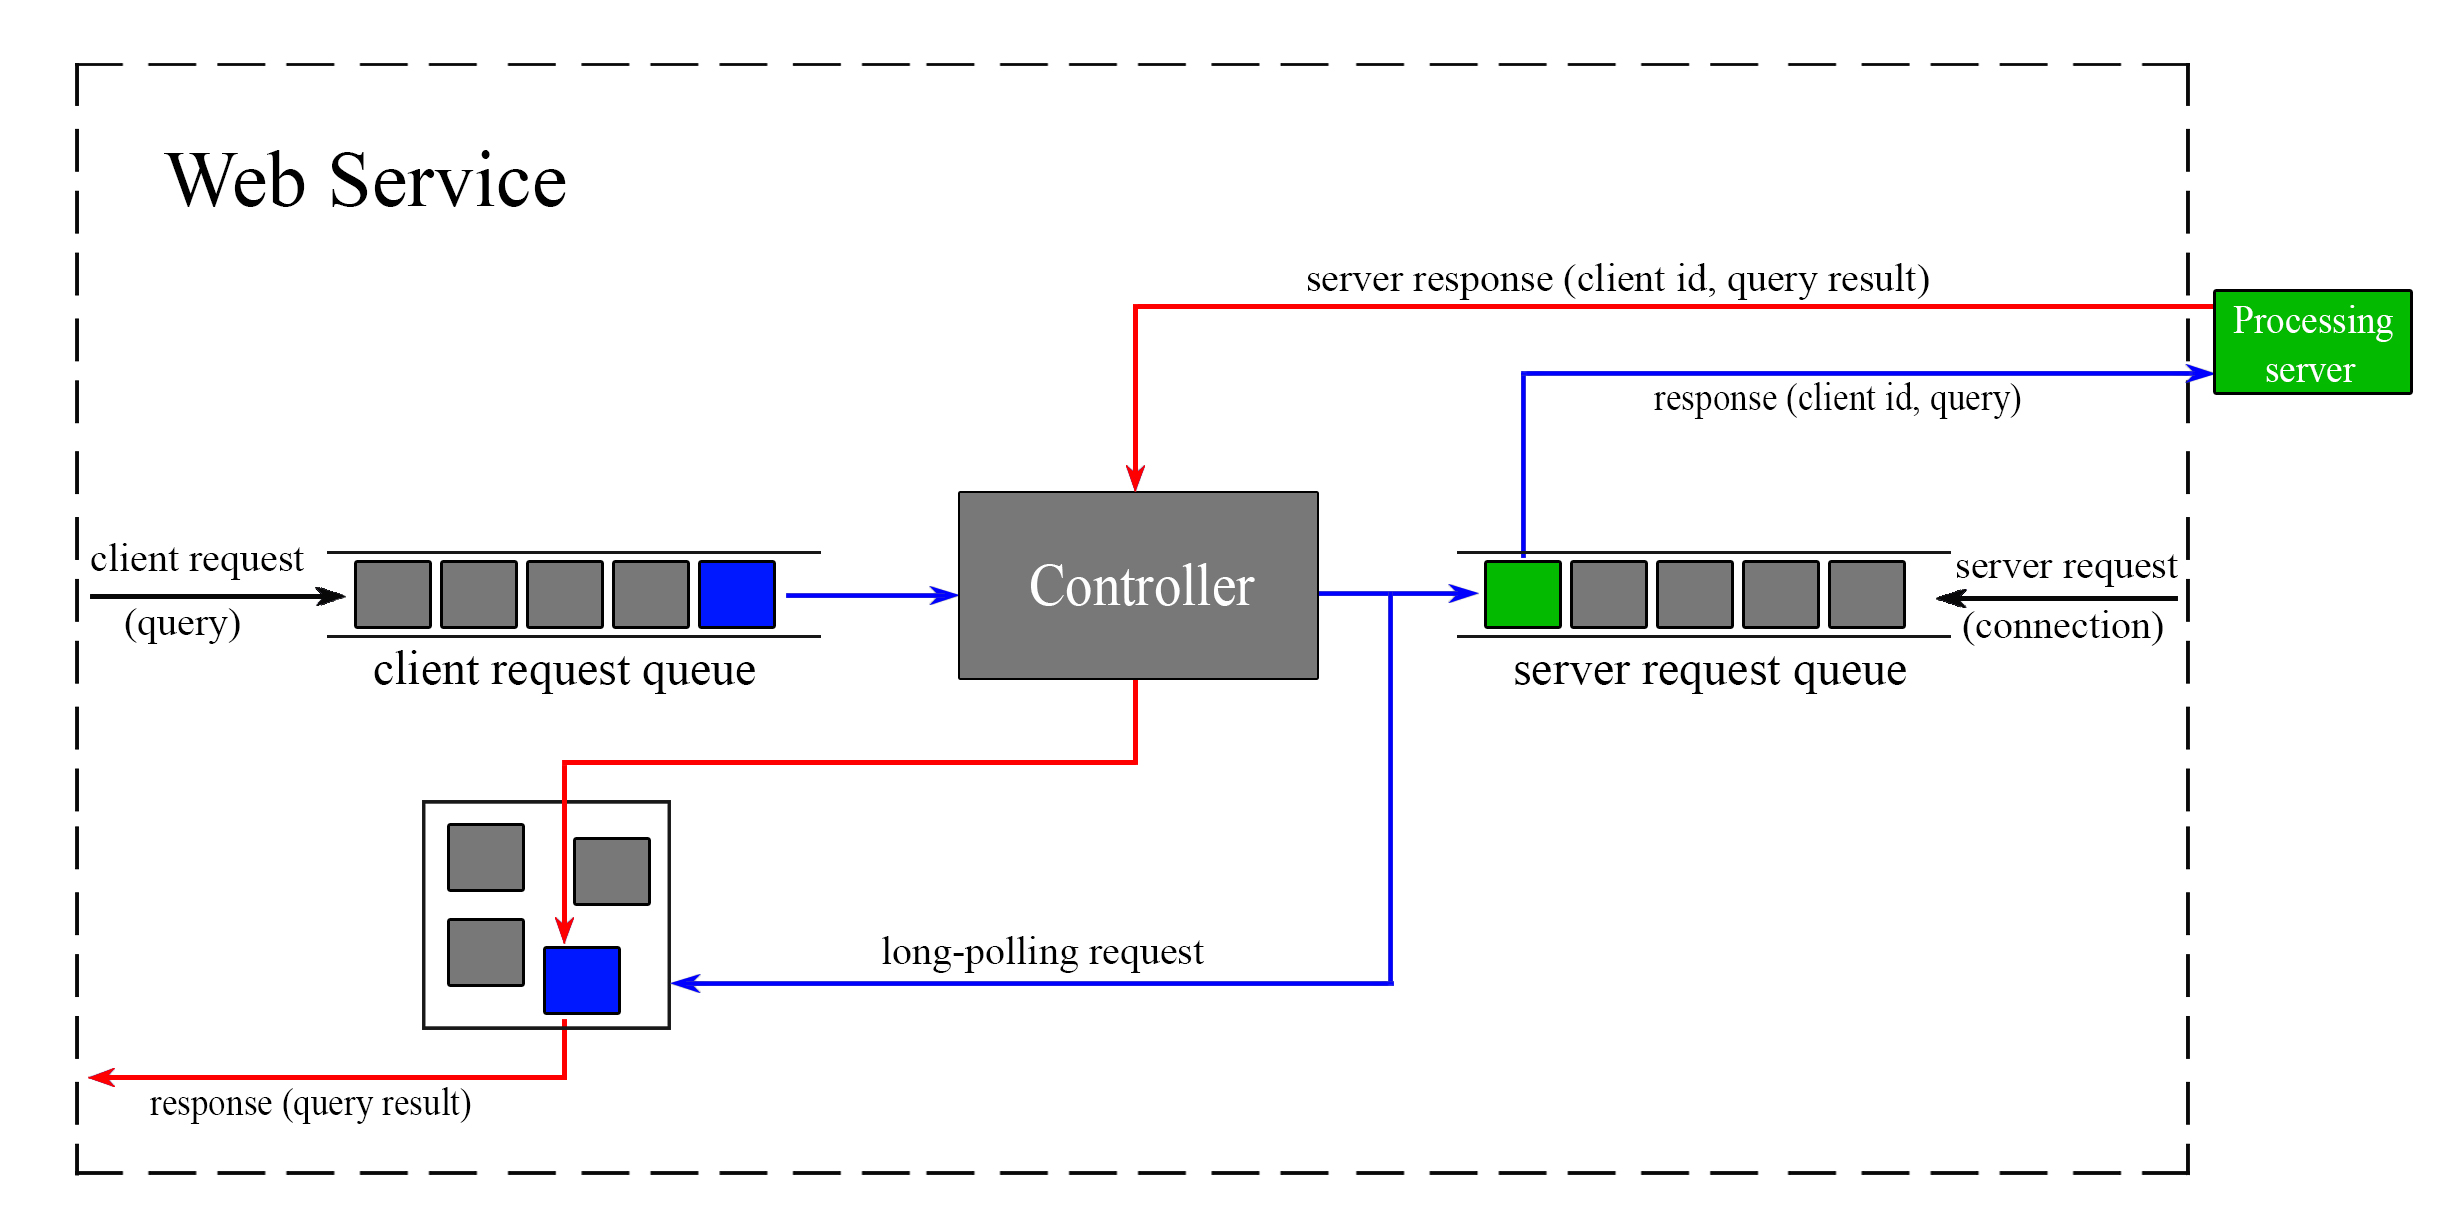
\includegraphics[scale=0.17]{ws_model}
    \fi
    \caption[Sơ đồ mô hình hoạt động chi tiết của web service]{Sơ đồ mô hình hoạt động chi tiết của web service.}
    \label{FigWS}
  \end{center}
\end{figure}

Trước tiên, mỗi yêu cầu do client gửi lên sẽ được đưa vào một hàng đợi. Đồng thời kết nối từ các server gửi lên cũng được đưa vào một hàng đợi để chờ client. Thành phần xử lý trung tâm là Controller sẽ lấy từng yêu cầu của client trả về cho một server đang chờ kết nối. Tiếp đó, yêu cầu của client sẽ bị giữ lại đề chờ kết quả xử lý từ phía server bằng kỹ thuật long-polling. Sau khi hoàn tất xử lý, server sẽ gửi lại web service kết quả xử lý cùng với thông tin client, từ đó web service sẽ đáp trả yêu cầu của client tương ứng.

\textbf{Kỹ thuật Long-polling.} Để client và server xử lý kết nối thời gian thực với nhau, chúng tôi xử dụng kỹ thuật long-polling là một kỹ thuật trong lập trình ứng dụng web. Một ví dụ đơn giản về kỹ thuật này là ứng dụng chat trên internet. Khi một user (1) gửi thông điệp chat tới một user khác (2) thông qua web service, nhưng web service không thể gửi thông điệp đó tới user 2. Khi đó user 2 phải liên tục gửi yêu cầu lên web service để xem có ai chat với mình hay không. Như vậy nếu muốn kết nối thời gian thực thì các user phải liên tục gửi yêu cầu liên web service, với số lượng lớn yêu cầu thì web service sẽ không thể đáp ứng nổi. Khi đó kỹ thuật long-polling được đưa ra nhằm giải quyết vấn đề này. Trong trường hợp trên, khi user 1 gửi yêu cầu lên web service, yêu cầu này sẽ không được trả về ngay lập tức mà nó bị giữ lại. Khi user 2 gửi thông điệp tới user 1 thì lúc này web service mới trả yêu cầu cùng thông điệp cho user 1. Cứ như thế 2 user có thể tương tác thời gian thực với nhau.

Trong hệ thống của chúng tôi, kỹ thuật long-polling được sử dụng để giữ yêu cầu kết nối của các server để chờ client, và giữ yêu cầu truy vấn của client để chờ kết quả xử lý từ server.

\subsection{Client side}
\label{subsection:client_side}
\subsubsection{Tổng quan}
Client side là một ứng dụng cung cấp giao diện để người dùng tương tác với hệ thống tìm kiếm. Nhận đầu vào là một hình ảnh cùng vùng đối tượng cần truy vấn, ứng dụng sẽ nén và mã hóa hình ảnh này sau đó gửi tới web service thông qua giao thức HTTP. Khi có kết quả trả về, ứng dụng sẽ phân tích và giải mã kết quả sau đó hiện thị cho người dùng. Hình \ref{FigAndroidClient} sau đây cho mô hình hoạt đổng tổng quan của ứng dụng tại client side.

\begin{figure}[!htbp]
  \begin{center}
    \leavevmode
    \ifpdf
      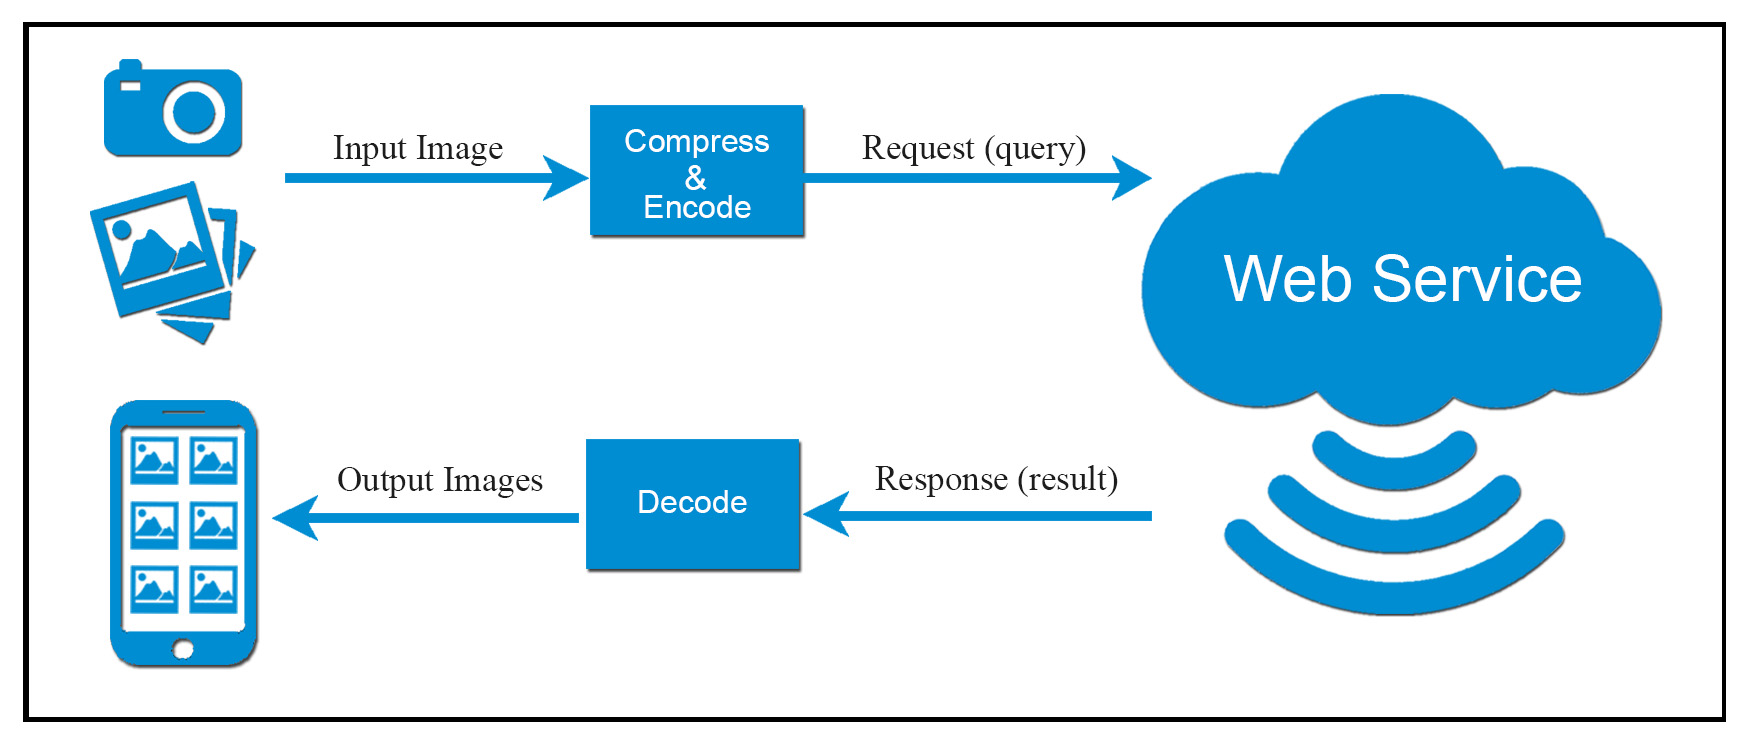
\includegraphics[scale=0.25]{android_client}
    \else
      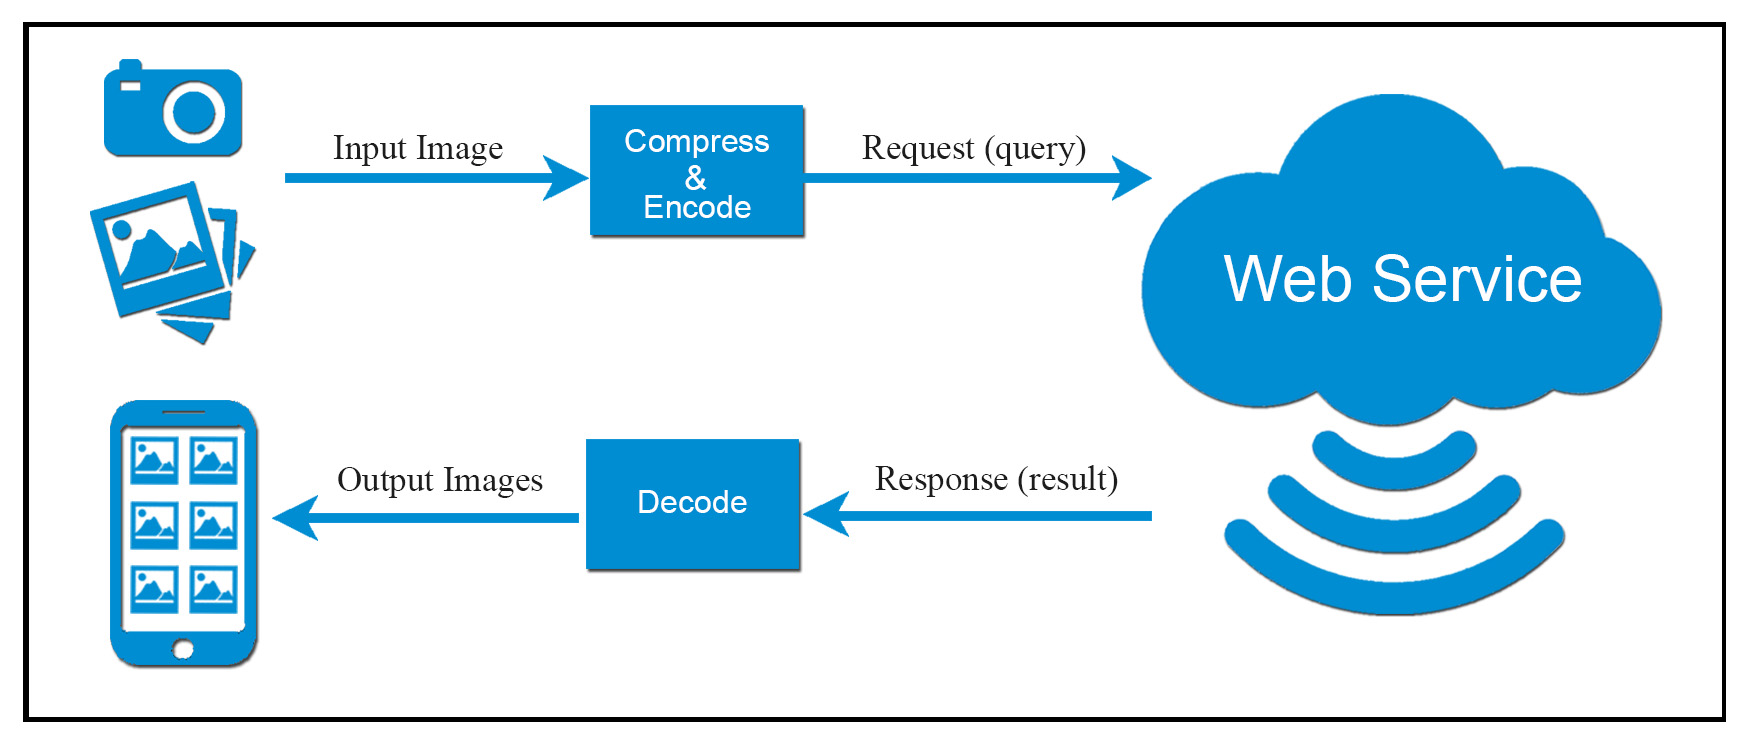
\includegraphics[scale=0.25]{android_client}
    \fi
    \caption[Kiến trúc của client side]{Kiến trúc của client side.}
    \label{FigAndroidClient}
  \end{center}
\end{figure}

Ứng dụng được xây dựng dành cho hệ điều hành Android, được viết bằng ngôn ngữ lập trình Java. Chi tiết tổ chức các lớp được thể hiện trong Hình \ref{FigClientFramework}.

\begin{figure}[!htbp]
  \begin{center}
    \leavevmode
    \ifpdf
      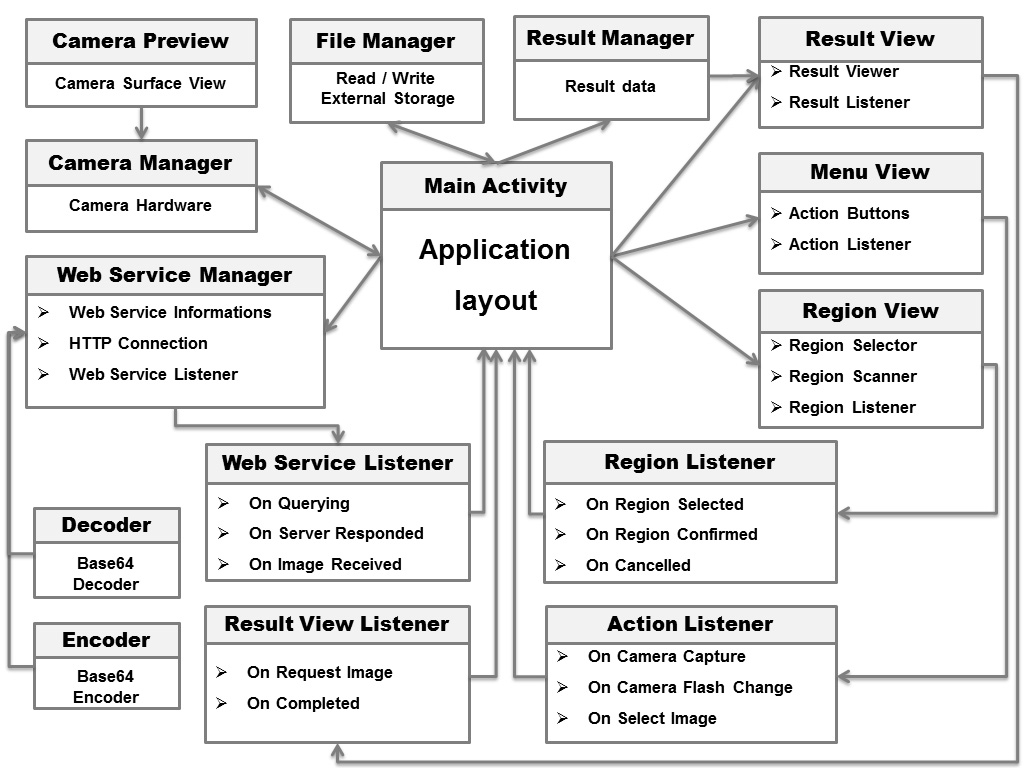
\includegraphics[scale=0.4]{client_model}
    \else
      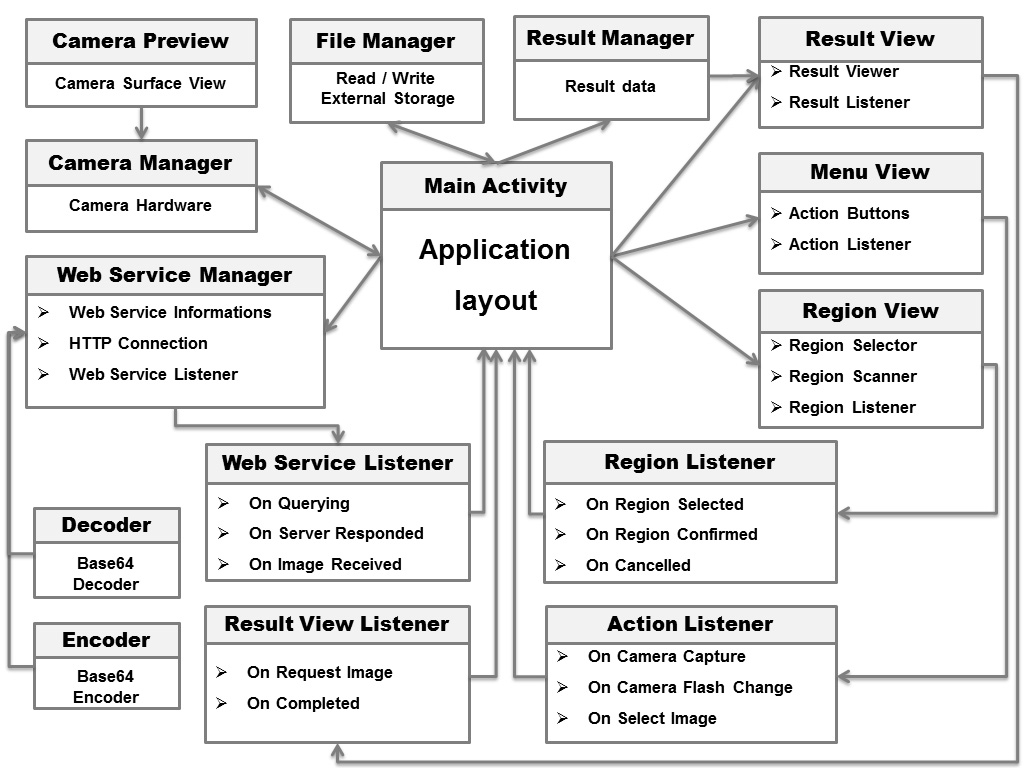
\includegraphics[scale=0.4]{client_model}
    \fi
    \caption[Sơ đồ tổ chức các lớp của ứng dụng trên hệ hệ điều hành Android.]{Sơ đồ tổ chức các lớp của ứng dụng trên hệ hệ điều hành Android.}
    \label{FigClientFramework}
  \end{center}
\end{figure}

%% trình bày chi tiết các lớp ...
\begin{itemize}
\item \textbf{Lớp CameraManager:} truy xuất tới camera trên điện thoại di động, thiết lập các thông số liên quan tới camera, nhận dữ liệu hình ảnh từ camera.

\item \textbf{Lớp WebServiceManager:} lưu trữ thông tin kết nối và thực hiện các kết nối tới web service, gửi và nhận dữ liệu truy vấn, gọi bộ interface lắng nghe sự kiện WebServiceListener để tương tác với các thành phần khác của ứng dụng.

\item \textbf{Lớp ResultManager:} nhận, lưu trữ và quản lý kết quả truy vấn.

\item \textbf{Lớp Decoder và Encoder:} giải mã và mã hóa hình ảnh. Để dễ dàng cho quá trình truyền dẫn dữ liệu giữa client, web service và server thì mỗi hình ảnh sẽ được mã hóa dưới dạng Base64 String.

\item \textbf{Interface WebServiceListener:} bộ lắng nghe các sự kiện liên quan tới web service. Onquerying: trong khi đang truy vấn. OnServerResponded: khi có kết quả phản hồi từ server, OnImageRecieved: khi có kết quả là các hình ảnh được trả về.

\item \textbf{Interface ResultViewListener:} bộ lắng nghe sự kiện liên quan tới việc hiển thị kết quả truy vấn. OnRequestImage: yêu cầu tải về một hình ảnh khi chọn xem hoặc tải xuống thiết bị, tải về danh sách hình ảnh khi người dùng muốn xem thêm kết quả. OnCompleted: khi hoàn tất việc xem kết quả, kết thúc một quá trình truy vấn.

\item \textbf{Interface ActionListener:} bộ lắng nghe các sự kiện là các chức năng trên ứng dụng. OnCameraCapture: khi có yêu cầu chụp hình. OnCameraFlashChange: khi có yêu cầu thay đổi trạng thái đèn flash. OnSelectImage: khi có yêu cầu chọn một hình ảnh trong thiết bị để truy vấn.

\item \textbf{Interface RegionListener:} bộ lắng nghe các sự kiện liên quan tới chức năng chọn vùng đối tượng trên camera. OnRegionSelected: khi người dùng đã chọn vùng đối tượng. OnRegionConfirmed: khi vùng đối tượng đã được xác nhận và được tiến hành truy vấn. OnRegionCancelled: Khi vùng đối tượng đã bị hủy.

\item \textbf{Lớp CameraPreview:} hiển thị dữ liệu được lấy từ camera.

\item \textbf{Lớp MenuView:} cung cấp các phím chức năng cho phép người dùng thao tác với ứng dụng, bao gồm phím chụp hình cho phép người dùng chụp hình ảnh để truy vấn, phím flash để người dùng thay đổi trạng thái đèn flash, phím chọn hình ảnh để người dùng chọn một hình ảnh trong thiết bị dùng làm hình ảnh truy vấn; gọi bộ lắng nghe sự kiện ActionListener khi người dùng thực hiện các chức năng để tương tác với các thành phần khác.

\item \textbf{RegionView:} cung cấp cho người dùng chức năng chọn vùng đối tượng trên camera. gọi bộ lắng ghe sự kiện RegionSelectionListener để tương tác với các thành phần khác.

\item \textbf{ResultView:} cung cấp giao diện cho phép người dùng xem và thao tác trên kết quả truy vấn, gọi bộ lắng nghe sự kiên ResultListener để thao tác với các thành phần khác.

\item \textbf{Lớp FileManager:} đọc, ghi dữ liệu từ bộ nhớ thiết bị.

\item \textbf{Lớp MainActitity:} cung cấp giao diện chính cho ứng dụng, là thành phần trung tâm quản lý toàn bộ các lớp khác, được cài đặt tất cả các bộ lắng nghe sự kiện để các lớp có thể giao tiếp với nhau thông qua nó.

\end{itemize}

\subsubsection{Chức năng và giao diện}
Là thành phần tương tác trực tiếp với người dùng, do đó ứng dụng cần đáp ứng các yêu cầu về giao diện thân thiện, đơn giản, tiện dụng nhưng vấn cung cấp đầy đủ các chức năng cho người dùng.

Dưới đây là giao diện cùng các chức năng của ứng dụng được thể hiện qua các hình \ref{FigInterface1}, \ref{FigInterface2}, \ref{FigInterface3}, \ref{FigInterface4}, \ref{FigInterface5} và \ref{FigInterface6}.
\\
\\
\begin{figure}[!htbp]
  \begin{center}
    \leavevmode
    \ifpdf
      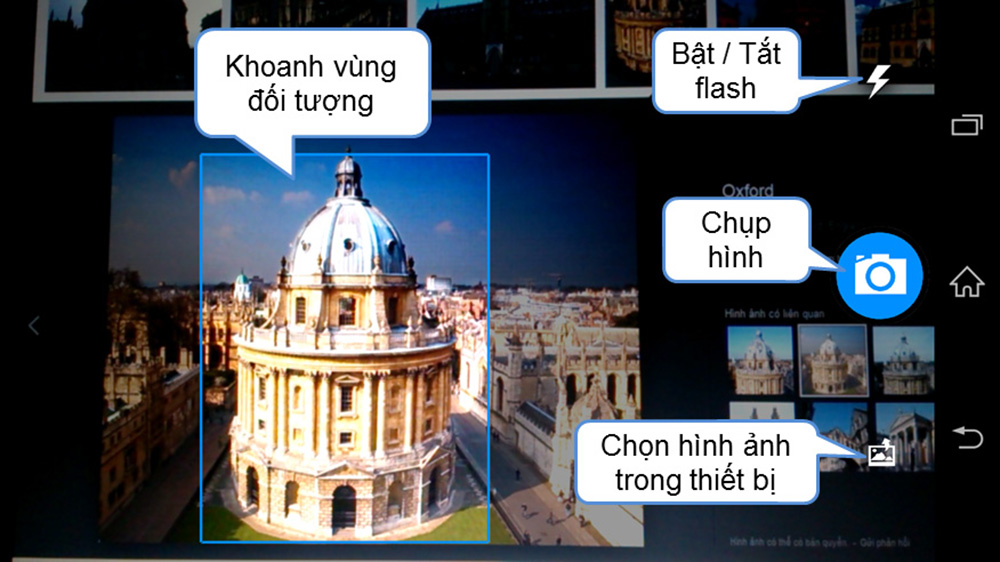
\includegraphics[scale=0.38]{interface_1}
    \else
      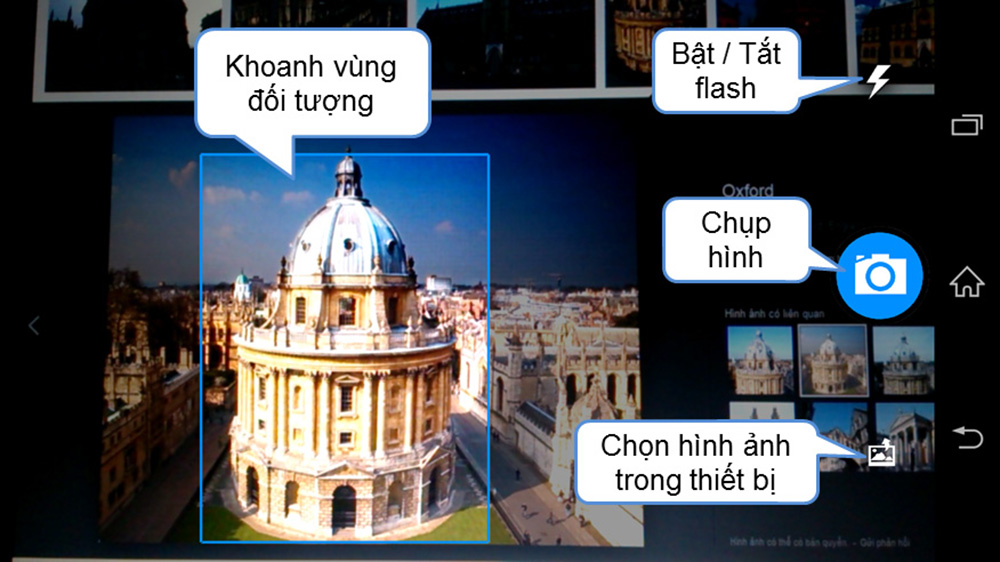
\includegraphics[scale=0.38]{interface_1}
    \fi
    \caption[Hình ảnh ứng dụng với các chức năng chính]{Hình ảnh giao diện ứng dụng với các chức năng chính. Ứng dụng cho phép người dùng chọn vùng đối tượng trên camera, chụp hình vùng đối tượng, bật / tắt đèn flash và chọn hình ảnh trong thiết bị để truy vấn.}
    \label{FigInterface1}
  \end{center}
\end{figure}
\\
\\
\begin{figure}[!htbp]
  \begin{center}
    \leavevmode
    \ifpdf
      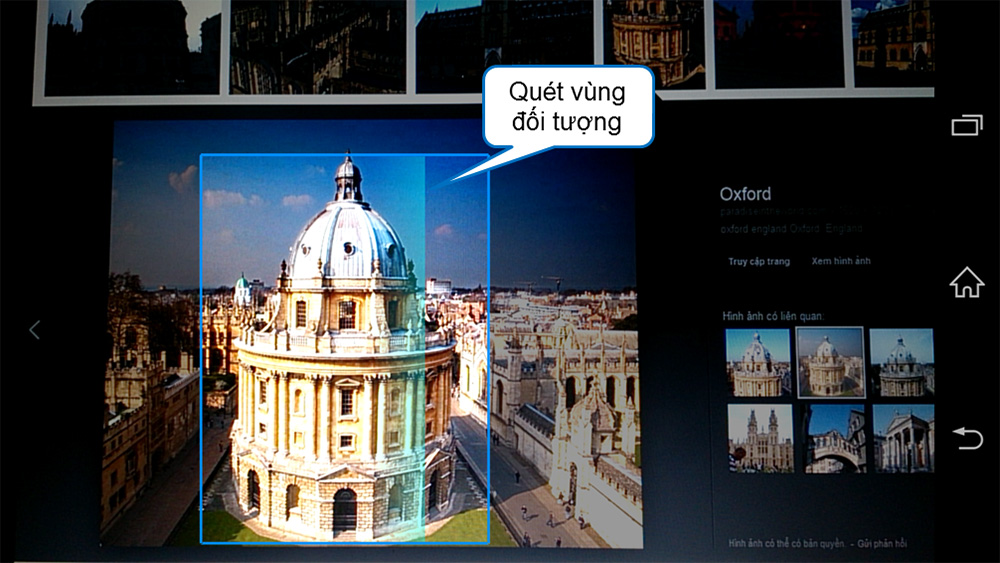
\includegraphics[scale=0.35]{interface_2}
    \else
      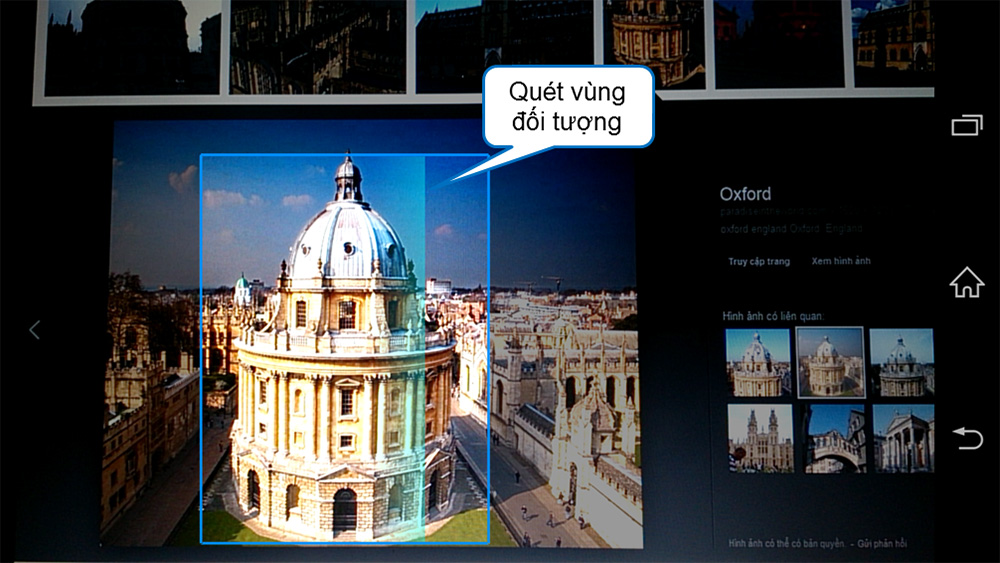
\includegraphics[scale=0.35]{interface_2}
    \fi
    \caption[Hình ảnh ứng dụng trong khi thực hiện truy vấn]{Hình ảnh ứng dụng trong khi thực hiện truy vấn. Trong khi chờ kết quả xử lý từ server, ứng dụng sẽ tạo hiệu ứng quét trên vùng đối tượng đã chọn để tránh cảm giác chờ đội. Tương tự khi chọn một hình ảnh trong thiết bị để truy vấn, ứng dụng cũng quét trên toàn bộ vùng truy vấn.}
    \label{FigInterface2}
  \end{center}
\end{figure}

\begin{figure}[!htbp]
  \begin{center}
    \leavevmode
    \ifpdf
      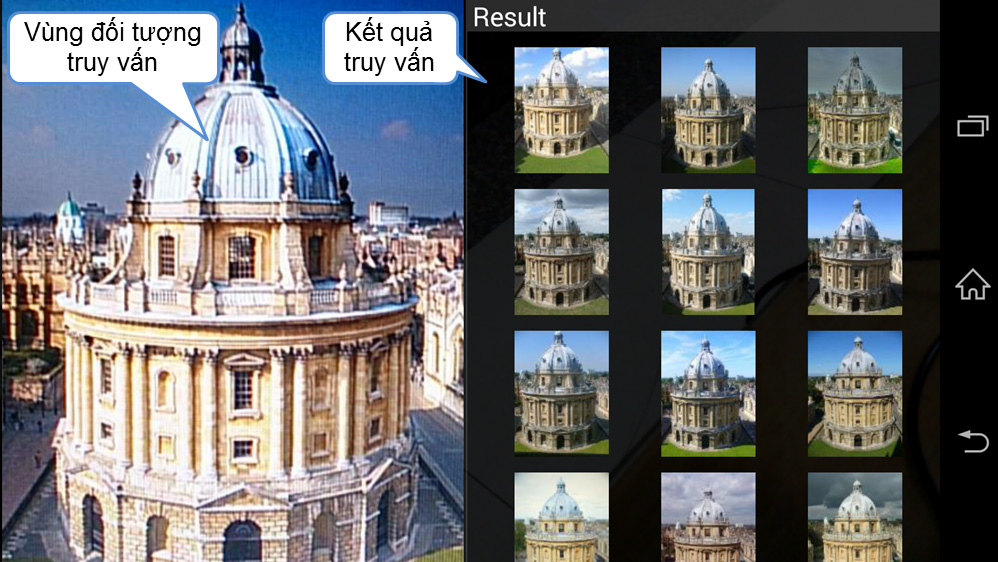
\includegraphics[scale=0.35]{interface_3}
    \else
      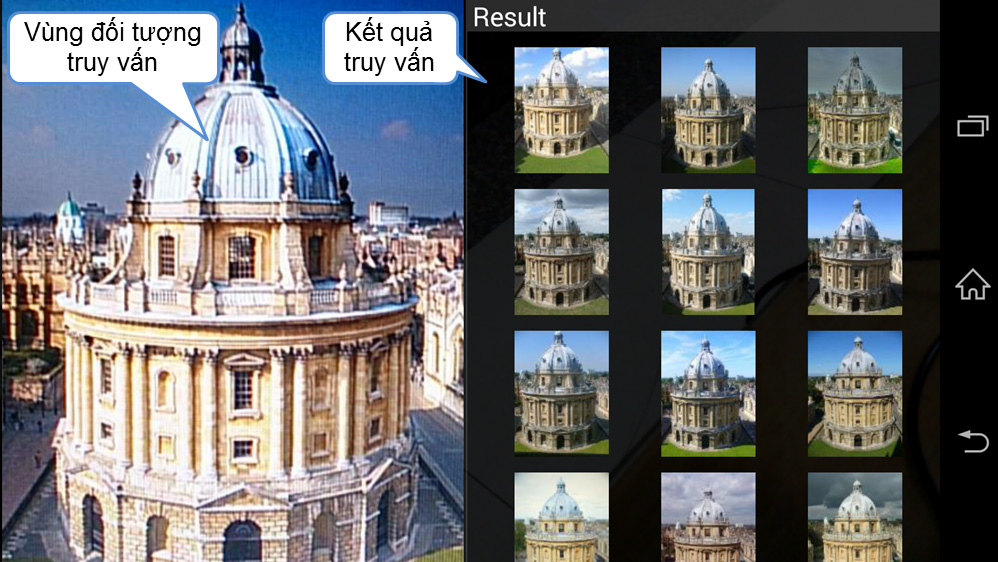
\includegraphics[scale=0.35]{interface_3}
    \fi
    \caption[Hình ảnh ứng dụng khi có kết quả trả về]{Hình ảnh ứng dụng khi có kết quả trả về. Ứng dụng cho người dùng xem vùng đối tượng vừa được truy vấn cùng danh sách các hình ảnh thu nhỏ được trả về từ server.}
    \label{FigInterface3}
  \end{center}
\end{figure}

\begin{figure}[!htbp]
  \begin{center}
    \leavevmode
    \ifpdf
      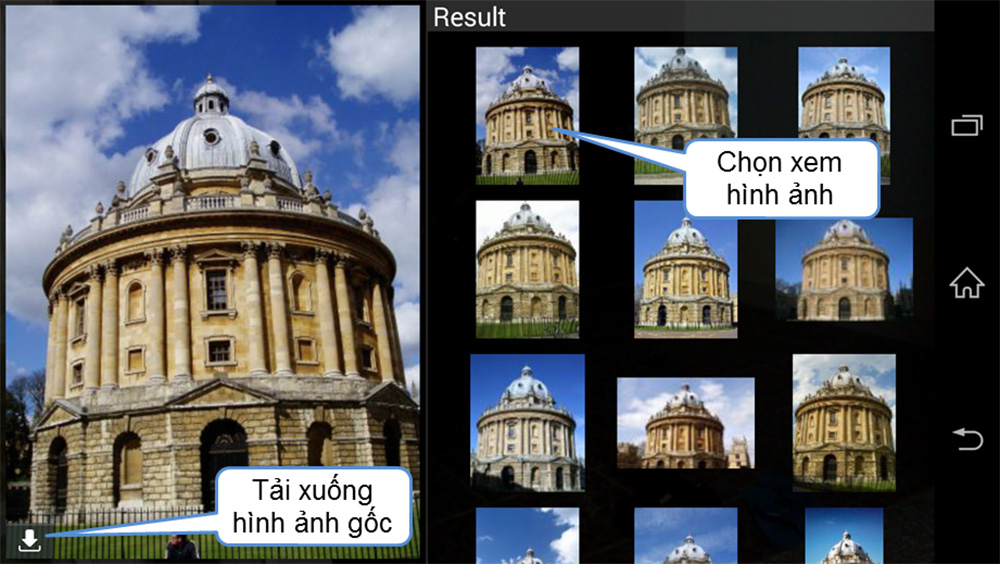
\includegraphics[scale=0.35]{interface_4}
    \else
      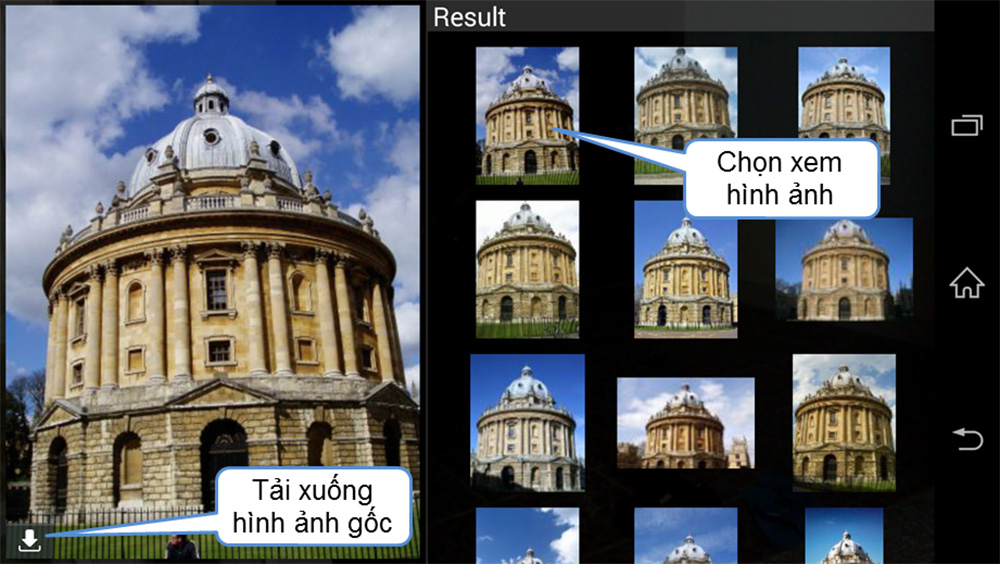
\includegraphics[scale=0.35]{interface_4}
    \fi
    \caption[Hình ảnh ứng dụng khi xem chi tiết kết quả truy vấn]{Hình ảnh ứng dụng khi xem chi tiết kết quả truy vấn. Người dùng có thể chọn xem một hình ảnh trong danh sách kết quả truy vấn. Ứng dụng sẽ tải hình ảnh chất lượng cao hơn để người dùng dễ dàng xem trong khung hình lớn hơn, nhưng đây chưa phải hình ảnh với chất lượng tốt nhất. Do dó, ứng dụng cũng cho phép người dùng tải hình ảnh gốc chất lượng cao bằng cách chạm vào nút như trên hình.}
    \label{FigInterface4}
  \end{center}
\end{figure}

\begin{figure}[!htbp]
  \begin{center}
    \leavevmode
    \ifpdf
      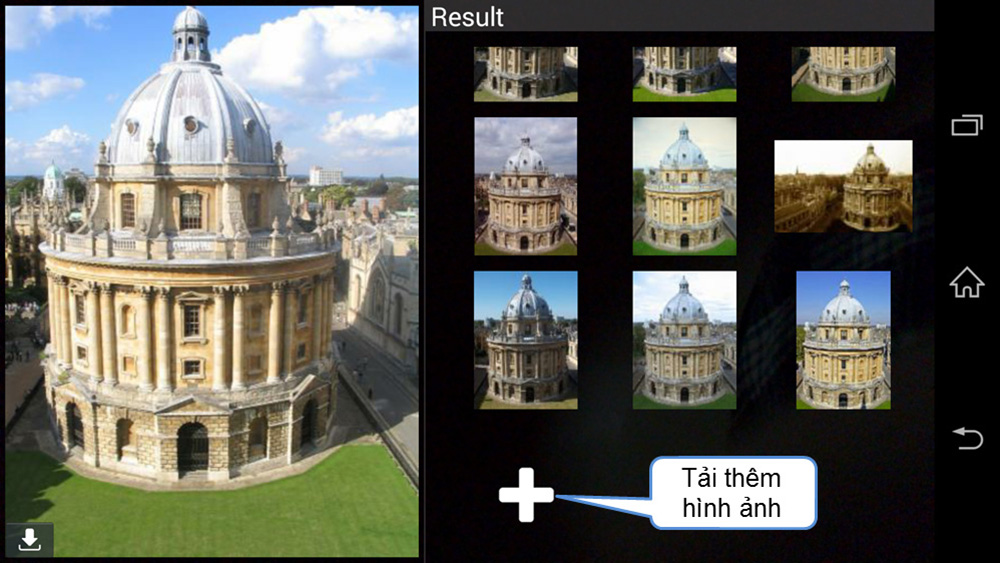
\includegraphics[scale=0.35]{interface_5}
    \else
      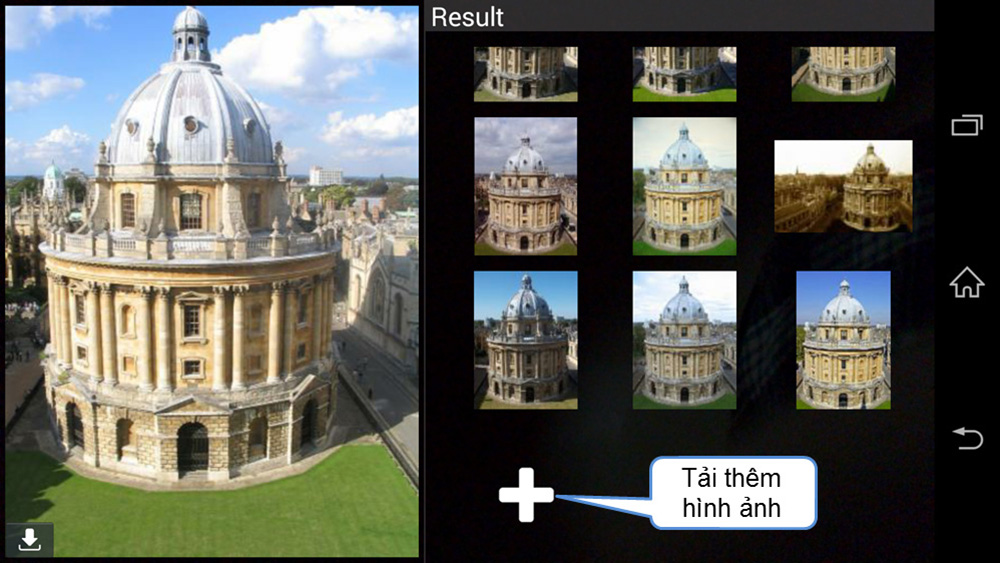
\includegraphics[scale=0.35]{interface_5}
    \fi
    \caption[Hình ảnh ứng dụng với chức năng tải thêm hình ảnh trong danh sách kết quả]{Hình ảnh ứng dụng với chức năng tải thêm hình ảnh trong danh sách kết quả truy vấn. Khi hoàn tất xử lý, server chỉ trả về cho ứng dụng một số hình ảnh đứng đầu danh sách xếp hạng, người dùng có thể tải thêm các hình ảnh khác bằng cách chạm vào dấu cộng như trên hình, với số lượng hình ảnh tối đa có thể tải là 50 hình.}
    \label{FigInterface5}
  \end{center}
\end{figure}

\begin{figure}[!htbp]
  \begin{center}
    \leavevmode
    \ifpdf
      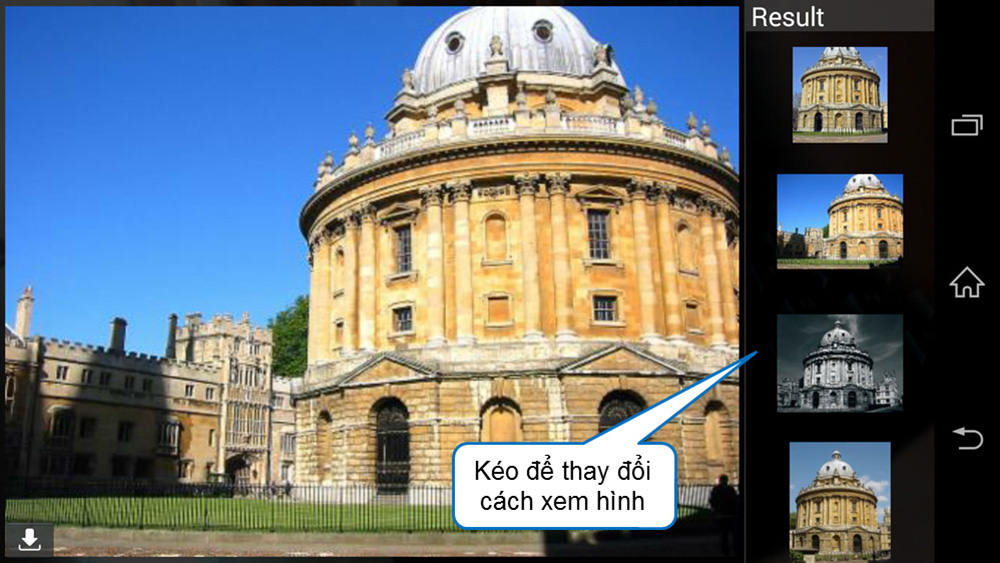
\includegraphics[scale=0.35]{interface_6}
    \else
      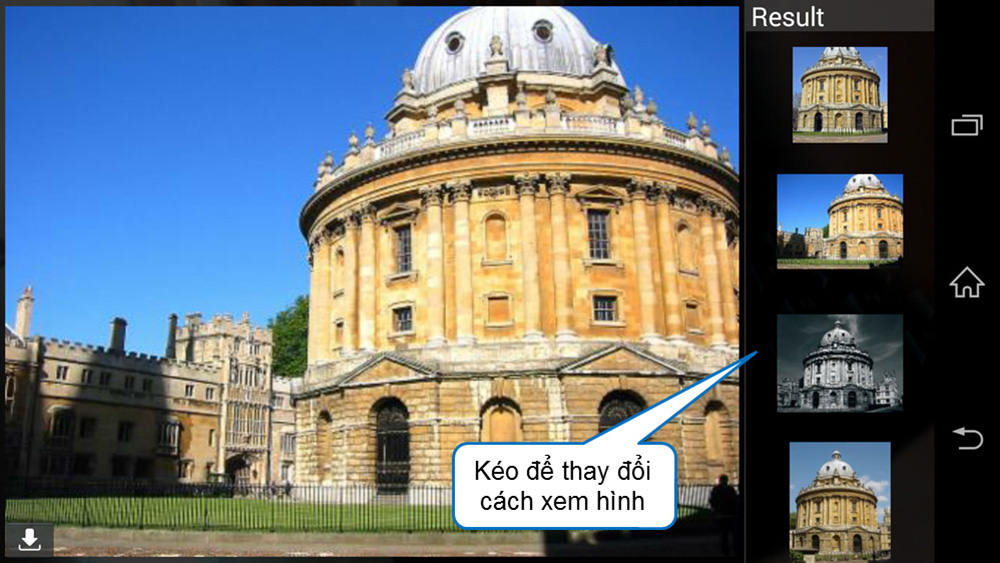
\includegraphics[scale=0.35]{interface_6}
    \fi
    \caption[Hình ảnh ứng dụng với chức năng thay đổi chế độ xem ảnh]{Ứng dụng cho phép người dùng thay đổi chế độ xem hình ảnh truy vấn bằng cách kéo khung kết quả để thu nhỏ, phóng to hình ảnh đang xem.}
    \label{FigInterface6}
  \end{center}
\end{figure}

\subsection{Tối ưu hiệu suất hệ thống}
\label{subsection:optimize}
Việc xử lý truy vấn hình ảnh đòi hỏi chi phí tính toán rất lớn, vì vậy một hệ thống tìm kiếm hình ảnh muốn đáp ứng được các yêu cầu thực tế cần phải tối ưu hóa hiệu suất trong quá trình xử lý cũng như truyền dẫn. Trong hệ thống đã xây dựng, chúng tôi đưa ra các giải pháp đề tối ưu hoạt động tại cả ba thành phần của hệ thống là client side, web service và sever side.

\begin{itemize}
\item \textbf{Tại client side: giảm tối đa dung lượng hình ảnh truy vấn}

Như đã trình bày trong mục \ref{subsection:web_service}, thời gian truyền dữ liệu dẫn phụ thuộc phần lớn vào tốc độ băng thông tại client, mà hình ảnh là dữ liệu khá lớn. Vì vậy chúng tôi đưa ra giải pháp giảm tối đa dung lượng hình ảnh nhưng vẫn đảm bảo kết quả truy vấn.

Dung lượng hình ảnh phụ thuộc vào ba yếu tố chính là kích thước ảnh, định dạng ảnh và chất lượng hình ảnh. Khi nhận được dữ liệu từ camera của điện thoại, hình ảnh sẽ được nén dưới định dạng JPEG ở mức chất lượng là 30\%, sau đó nó sẽ được điều chỉnh lại với kích thước tối đa là 500 x 500 pixel. Ví dụ, một hình ảnh được chụp từ điện thoại với độ phân giải 2 Megapixel (1920x1080) có dung lượng khoảng 500 kilobytes (kB), sau khi được nén dưới định dạng JPEG ở mức chất lượng 30\% và điều chỉnh kích thước xuống 500x281 pixel, dung lượng hình ảnh giảm chỉ còn khoảng 15kB, tức là giảm 97\%. Như vậy, việc truyền tải sẽ rất nhanh chóng, có thể đáp ứng được trên mạng EDGE với tốc độ 236kb/s. Nhưng với chất lượng hình ảnh như vậy sẽ ảnh hưởng tới kết quả truy vấn.

Kết quả truy vấn phụ thuộc phần lớn vào quá trình trích xuất đặc trưng tại server xử lý, và chất lượng hình ảnh sẽ ảnh hưởng trực tiếp tới quá trình này. Tại bước trích xuất đặc trưng, server xử lý sử dụng bộ phát hiện đặc trưng Hessian-Affine\cite{mikolajczyk2005comparison} detector và bộ mô tả đặc trưng SIFT descriptor\cite{lowe2004distinctive}, cả hai đều phụ thuộc phần lớn vào texture trên hình ảnh là các góc cạnh, đường viền. Việc giảm dung lượng hình ảnh như đã trình bày ở trên không làm mất các góc cạnh đường viền trên hình, vì vậy không ảnh hưởng nhiều tới kết quả truy vấn, mặt khác nó còn giúp tăng tốc độ xử lý trích xuất đặc trưng tại phía server.

\item \textbf{Tại web service: giảm số lượng request bằng kỹ thuật long-polling}

Kỹ thuật long-polling như đã trình bày trong mục \ref{subsection:web_service} giúp giảm lượng request từ mỗi client khi có yêu cầu truy vấn hình ảnh. Vì vậy hệ thống có thể đáp ứng được nhiều request hơn, tốc độ phản hồi tới client vì thế cũng sẽ nhanh hơn.

\item \textbf{Tại server xử lý: sử dụng phương pháp đề xuất và tối ưu kết quả trả về}

Để tăng tốc độ truy vấn, hệ thống xử dụng phương pháp đề xuất đã trình bày trong mục \ref{sec:intergrated} cùng những kết quả thí nghiệm chứng minh tính hiệu quả của phương pháp trong chương \ref{chapter:experiment}. Cùng với đó là việc tối ưu kết quả trả về để giảm tối đa thời gian phản hồi tới client.

Kết quả của quá trình truy vấn là một danh sách các hình ảnh và việc trả về những hình ảnh này cho client cũng sẽ chịu ảnh hưởng rất lớn từ tốc độ băng thông. Với một yêu cầu truy vấn, server chỉ cần trả về một số hình ảnh đầu trong danh sách xếp hạng là đủ, và chỉ trả về các hình ảnh thu nhỏ dể giảm tối đa thời gian phản hồi về client. Cụ thể hơn, khi có kết quả truy vấn, server sẽ trả về cho client 15 hình ảnh thu nhỏ đứng đầu danh sách xếp hạng, mỗi hình thu nhỏ này có kích thước tối đa là 150 x 150 pixel và kích cỡ trung bình khoảng 5kB mỗi hình. Như vậy, tổng dung lượng cần gửi về client cho mỗi lần truy vấn là khoảng 75kB, vẫn có thể đáp ứng trên những kết nối chậm. 

Thêm vào đó, việc sử dụng các server truy xuất dữ liệu độc lập với quá trình xử lý truy vấn cũng giúp tăng hiệu suất của hệ thống bằng cách phàn hồi từng phần dữ liệu về client. Với chức năng xem cụ thể hình ảnh trả về, các server truy xuất dữ liệu sẽ nhận yêu cầu xem hình ảnh từ client và gửi về một hình ảnh thu nhỏ với kích thước tối đã là 500 x 500 pixel, với dung lượng khoảng 30kB mỗi hình, vẫn có thể hiển thị tốt trên điện thoại di động màn hình Full HD (1920x1080) trong khi dung lượng giảm tới 95\% (với bộ dữ liệu oxford 5k, mỗi hình ảnh gốc nặng trung bình 500kB).

\end{itemize}

Hiệu quả của việc tối ưu các thành phần trên sẽ được kiểm chứng trong phần tiếp theo.

\section{Cài đặt và thực nghiệm}
\label{c5-caidat}
	\subsection{Môi trường cài đặt}
	Môi trường cài đặt của hệ thống được liệt kê chi tiết dưới đây:
	
	\begin{itemize}
	\item \textbf{Processing Server:}
	
	-- Hệ điều hành: Windows Server 2008.
	
	-- Ngôn ngữ lập trình: Matlab, C, Java.
	
	\item \textbf{Web Service:}
	
	-- Web server: Apache Tomcat 7.
	
	-- Ngôn ngữ lập trình: Java.
	
	\item \textbf{Client:}
	
	-- Hệ điều hành: Android 4.0.
	
	-- Ngôn ngữ lập trình: Java. 
	\end{itemize}	
	
	\subsection{Kết quả thực nghiệm và đánh giá ứng dụng}
	Chúng tôi đánh giá ứng dụng dựa trên hai yếu tố chính: giao diện người dùng và hiệu suất truy vấn.
	
	Về giao diện người dùng, ứng dụng thể hiện tính thân thiện cao và dễ sử dụng, cung cấp cho người dùng đủ các tính năng cơ bản của một hệ thống tìm kiếm hình ảnh.
	
	Để đánh giá hiệu suất truy vấn, chúng tôi đo \textbf{thời gian phản hồi} của một truy vấn cơ bản, tính từ khi client gửi yêu cầu truy vấn tới khi nhận được kết quả, thực hiện trên bộ dữ liệu chuẩn Oxford Buildings 5k (Bảng \ref{table:datasets}). Thêm vào đó, để đánh giá chi tiết hơn, chúng tôi cũng đo các thông số sau:
	
	-- Dung lượng (DL) hình ảnh truy vấn sau mã hóa (MH).
	
	-- Thời gian xử lý tại client và server: tại client, thời gian xử lý là thời gian nén và mã hóa hình ảnh truy vấn và giải mã kết quả. Tại server, thời gian xử lý bao gồm: trích xuất đặc trưng (TXĐT), truy vấn, giải mã (GM) và mã hóa (MH) và truy xuất dữ liệu (TXDL).
	
	-- Tổng thời gian truyển tải: Tổng chi phí thời gian truyền tải dữ liệu giữa client, web service và server xử lý cho một truy vấn cơ bản.
	
	-- Tổng dung lượng kết quả trả về.
	
\begin{figure}[!htbp]
  \begin{center}
    \leavevmode
    \ifpdf
      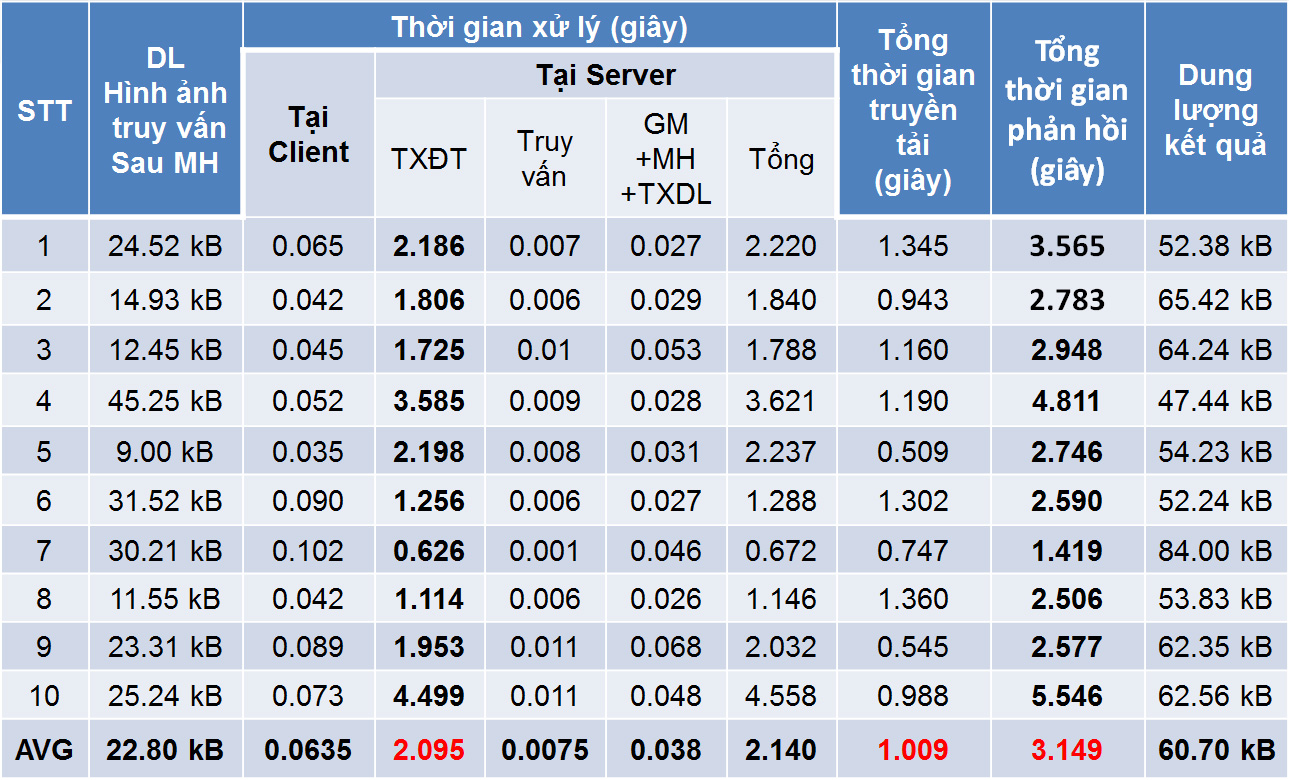
\includegraphics[scale=0.3]{app_experimental}
    \else
      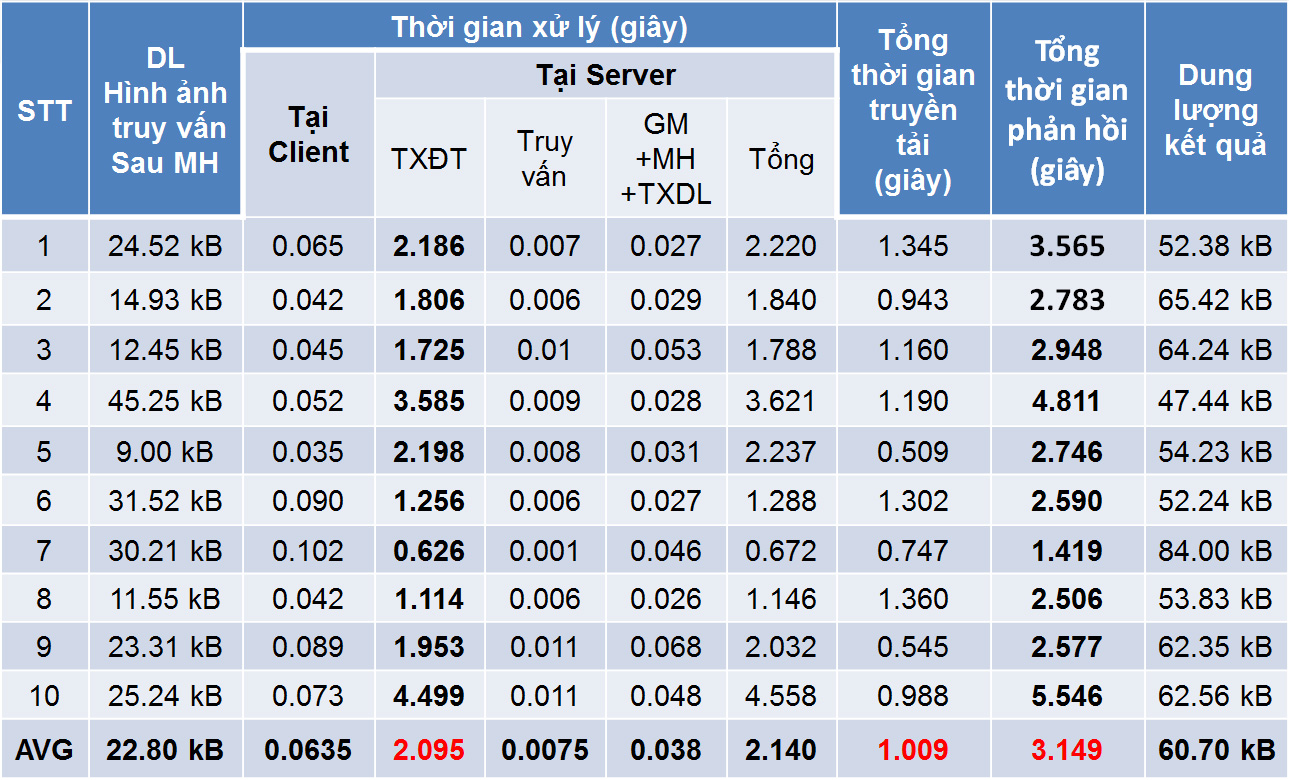
\includegraphics[scale=0.3]{app_experimental}
    \fi
    \caption[Kết quả thực nghiệm hiệu suất của hệ thống tìm kiếm đối tượng trên ảnh.]{Kết quả thực nghiệm hiệu suất của hệ thống tìm kiếm đối tượng trên ảnh.}
    \label{FigAppExperimental}
  \end{center}
\end{figure}
		
	Bảng \ref{FigAppExperimental} thể hiện kết quả thực nghiệm trên 10 truy vấn với các hình ảnh khác nhau được chụp trực tiếp trên điện thoại di động, kết nối với server thông qua mạng wifi cá nhân. Có thể thấy tổng thời gian phản hồi của một truy vấn phụ thuộc rất lớn vào thời gian xử lý tại server, cụ thể hơn là thời gian trích xuất đặc trưng. Với kết quả trên, thời gian trích xuất đặc trưng trung bình là 2.095 giây, chiếm 66.5\% tổng thời gian phản hồi, hơn nữa với những hình ảnh có độ phức tạp đặc trưng cao như hình truy vấn thứ 10 trong bảng \ref{FigAppExperimental}, thời gian trích xuất đặc trưng chiếm tới hơn 80\%. Điều này cũng dễ hiểu vì bước trích xuất đặc trưng sử dụng giải thuật phát hiện và mô tả đặc trưng khá phức tạp, là quá trình ảnh hưởng lớn nhất tới kết quả truy vấn.
	
	Trong khi đó, thời gian truyền tải trung bình cho toàn bộ quá trình là 1.009 giây, phụ thuộc chủ yếu vào tốc độ mạng của người dùng. Với dữ liệu gồm nhiều hình ảnh thì kết quả này là khá tốt, thể hiện hiệu suất của ứng dụng tại các bước nén và mã hóa hình ảnh, tối ưu quá trình truyền dẫn. Với tổng lưu lượng truyền dẫn cho cả quá trình là 85.6kB (dung lượng hình ảnh truy vấn và tổng dung lượng kết quả trả về) hoàn toàn có thể đáp ứng những kết nối chậm, chẳng hạn mạng EDGE với tốc độ 236kb/s.
	
	Kết quả truy vấn trung bình cho mỗi hình ảnh trong thí nghiệm trên là 7.5 ms, gần như không đáng kể,  cho thấy hiệu suất trong việc cải thiện tốc độ phản hồi của phương pháp đề xuất.
	
	Cũng có thể thấy thời gian xử lý giải mã, mã hóa và truy xuất file tại cả client và server là không đáng kể.
	
	Ngoài ra, một yếu tố quan trọng để đánh giá hiệu suất của ứng dụng là độ chính xác truy vấn. Ứng dụng sử dụng phương pháp đề xuất đã được trình bày trong mục \ref{chapter:proposed} và kết quả đã được thí nghiệm trên các bộ dữ liệu chuẩn tại mục \ref{chapter:experiment}. 
	
	Như vậy, những thực nghiệm trên cho thấy ứng dụng hoàn toàn có thể đáp ứng được các yêu cầu thực tế của một hệ thống tìm kiếm đối tượng trên ảnh.